\documentclass[11pt,a4paper]{article}
\usepackage{acl2015}
\usepackage[usenames,dvipsnames]{color}
\usepackage{times}
\usepackage{url}
\usepackage{latexsym}
\usepackage{amsmath}
\usepackage{ifthen}
\usepackage{xspace}
\usepackage{booktabs}
\usepackage{algorithm}
\usepackage{algorithmicx}
\usepackage{scalerel}
\usepackage{array}
\usepackage[noend]{algpseudocode}
\usepackage{tikz}
\usepackage[all]{nowidow}
\usetikzlibrary{trees,matrix,backgrounds}
\usepackage{afterpage}
\usepackage{multirow,color}
\usepackage{subcaption}
\usepackage{todonotes}

\newcommand{\trevor}[1]{{\color{Maroon}{\bf{Trevor says:}} \emph{#1}}}
\newcommand{\matthias}[1]{{\color{RedOrange}{\bf{Matthias says:}} \emph{#1}}}
\newcommand{\ehsan}[1]{{\color{Cerulean}{\bf{Ehsan says:}} \emph{#1}}}
\newcommand{\reza}[1]{{\color{Blue}{\bf{Reza says:}} \emph{#1}}}

\newcommand{\supp}{\emph{Supplementary Materials}\xspace}

\newcommand*\Let[2]{\State #1 $\gets$ #2}
\newcommand*\CSA{\textsc{Csa}\xspace}
\newcommand*\CST{\textsc{Cst}\xspace}
\newcommand*\CSTs{\textsc{Cst}s\xspace}
\algrenewcommand\algorithmicrequire{\textbf{Precondition:}}
\algrenewcommand\algorithmicensure{\textbf{Postcondition:}}

\newcommand{\ngram}{$m$gram\xspace}
\newcommand{\ngrams}{$m$grams\xspace}

\newcommand{\rooot}[1]{\text{root}(#1)}
\newcommand{\leaf}[2]{\text{leaf}(#1, #2)}
\newcommand{\size}[2]{\text{size}(#1, #2)}
\newcommand{\depth}[2]{\text{depth}(#1, #2)}
\newcommand{\degree}[2]{\text{degree}(#1, #2)}
\newcommand{\edge}[3]{\text{edge}(#1, #2, #3)}
\newcommand{\children}[2]{\text{children}(#1, #2)}
\newcommand{\parent}[2]{\text{parent}(#1, #2)}
\newcommand{\backwardsearch}[4]{\text{backward-search}(#1, [#2,#3], #4)}
\newcommand{\forwardsearch}[4]{\text{forward-search}(#1, [#2,#3], #4)} % I've abbreviated away depth, char_pos
\newcommand{\intervalsymbols}[3]{\text{interval-symbols}(#1, [#2,#3])}
\newcommand{\pathlabel}[2]{\text{label}(#1, #2)}

\DeclareMathOperator*{\Bigcdot}{\scalerel*{\cdot}{\bigodot}}

\newcommand{\lb}[1]{\text{lb}(#1)}
\newcommand{\rb}[1]{\text{rb}(#1)}
\newcommand{\dotpat}{\Bigcdot \alpha}
\newcommand{\patdot}{\alpha \Bigcdot}
\newcommand{\dotpatdot}{\Bigcdot \alpha \Bigcdot}
\newcommand{\nlplus}[1]{N^{1+}(#1)} % note it's an little L not a 1
\newcommand{\nlplusfunc}[3]{\textsc{N1Plus}(#1, #2, #3)} % "
\newcommand{\nlplusbacklfunc}[3]{\textsc{N1PlusBack1}(#1, #2, #3)} % " ^ 2
\newcommand{\nlplusfrontbackfunc}[4]{\textsc{N1PlusFrontBack}(#1, #2, #3, #4)} % " 
\newcommand{\nlplusfrontbacklfunc}[3]{\textsc{N1PlusFrontBack1}(#1, #2, #3)} % "

\newcommand{\tf}{t_{\text{F}}}
\newcommand{\tr}{t_{\text{R}}}
\newcommand{\af}{a_{\text{F}}}
\newcommand{\ar}{a_{\text{R}}}
\newcommand{\nf}{v_{\text{F}}}
\newcommand{\nr}{v_{\text{R}}}
\newcommand{\nrfull}{v_{\text{R}}^{\text{all}}}
\newcommand{\nffull}{v_{\text{F}}^{\text{all}}}
\newcommand{\chf}{u_{\text{F}}}
\newcommand{\chr}{u_{\text{R}}}

\newcommand{\ws}{\textbf{w}}

\newcommand{\Order}[1]{O(#1)}

%-- Sizes
\newcommand\kb[1]{\mbox{$#1$\,kiB}}
\newcommand\mb[1]{\mbox{$#1$\,MiB}}
\newcommand\gb[1]{\mbox{$#1$\,GiB}}
\newcommand\tb[1]{\mbox{$#1$\,TiB}}

%-- Syms
\newcommand{\col}{\ensuremath{\mathcal{T}}}  % collection
\newcommand{\pattern}{\ensuremath{\mathcal{P}}}  % collection
\newcommand{\plen}{\ensuremath{m}}
\newcommand{\collen}{\ensuremath{n}} 
\newcommand{\alphabet}{\ensuremath{\Sigma}} 
\newcommand{\alphabetsize}{\ensuremath{\sigma}} 


%-- ALG/DS
\newcommand{\SA}{\mbox{\emph{SA}}\xspace}


%%% Local Variables: 
%%% mode: latex
%%% TeX-master: "cstlm"
%%% End: 


% some mild cheats
\addtolength{\dbltextfloatsep}{-1ex}
\addtolength{\dblfloatsep}{-1ex}
\addtolength{\abovecaptionskip}{-1ex}
\addtolength{\belowcaptionskip}{-1ex}

\title{Compact, Efficient and Unlimited Capacity:
    Language Modeling with Compressed Suffix Trees}

\author{First Author \\
  Affiliation / Address line 1 \\
  Affiliation / Address line 2 \\
  Affiliation / Address line 3 \\
  {\tt email@domain} \\\And
  Second Author \\
  Affiliation / Address line 1 \\
  Affiliation / Address line 2 \\
  Affiliation / Address line 3 \\
  {\tt email@domain} \\}

\date{}

\begin{document}
\maketitle
\begin{abstract}
  Efficient methods for storing and querying langugage models are critical for scaling to large corpora and high Markov orders.
%While most previous work has focussed on efficient means of indexing \ngrams using a fixed, low Markov order,
In this paper we propose methods for modelling extremely large corpora without
imposing a Markov condition.
At its core, our approach uses a succinct index -- a \emph{compressed suffix tree} backed by a \emph{FM index} -- which provides near optimal compression while supporting efficient search.
We present algorithms for on-the-fly computation of probabilities under a
%n infinite order
Kneser-Ney language model.
Our technique is \emph{exact} and although slower than leading LM
toolkits, it shows promising scaling properties,
which we demonstrate through $\infty$-order modelling over the full Wikipedia collection. 


%%% Local Variables: 
%%% mode: latex
%%% TeX-master: "cstlm"
%%% End: 

\end{abstract}

\section{Introduction}
\label{sec-intro}
%Language modelling is the task of estimating the probability of sequences of words in a language.
Language models (LMs) are one of the major and large components in many modern NLP systems, 
e.g. machine translation \cite{koehn2010book} 
and automatic speech recognition \cite{rab93book}.
%
One approach for accurate language modeling is neural 
\cite{Bengio:2003:NPL,DBLP:conf/interspeech/MikolovKBCK10}, but another is  count-based 
\cite{chen1996empirical} to harness the power of more data.
%
%The predominant approach to count-based language modelling is the $n$gram model,
%where a typical LM can contain as many as several hundred billions of $n$grams XX.
%
To be useful, LMs need to be not only accurate but also fast and compact.
%
In this paper, we build  fast and compact high-order \ngram LMs
%, the predominant approach in count-based language modeling, 
using modern succinct data structures.

%where the probability of a sequence of words is decomposed based on the chain rule ad approximatedusing the Markov assumption XX. 
%A typical count-based LM can contain as many as several hundred billions of $n$grams
%In this paper, we build  fast and compact $n$gram LMs, the predominant approach in count-based language modeling, on web-scale corpora using modern succinct data structures.
%
%We show how to compactly index the text statistics needed by $n$gram language models, so that they can be queried efficiently to make the probabilities on the fly.       
%
%Importantly, the stored index and text statistics are kept intact for $n$gram LMs with different orders (i.e. the context size), hence allow to relax the
%Markov assumption made in these LMs by considering very large contexts.



Depending on the order and the training corpus size, a typical \ngram LM may contain as many as several hundred billions of \ngrams \cite{brants2007large},
so storage and query time become challenge.
%
As always, there is a trade-off between accuracy, space, and time, with recent papers considering small but approximate  \emph{lossy} LMs 
\cite{Chazelle:2004:BFE:982792.982797,guthrie2010storing},
or \emph{loss-less}  not-small LMs \cite{stolcke2011srilm} where compression and tries 
\cite{Germann:2009:TPT:1621947.1621952,heafield2011kenlm,pauls2011faster}, 
suffix trees \cite{kennington2012suffix}, and LODUS trees 
\cite{sall11,DBLP:conf/acl/WatanabeTI09}  
have been used to further reduce the storage.
% 
However, none of these papers scale up to high-order  
\ngram LMs on medium to web-scale corpora due to their large  memory footprints.
%
%However, none of the state-of-the-art LM toolkits provides the opportunity of
%investigating the behaviour of high-order LMs  
% 
Being able to work with high-order  LMs and investigate their behaviour 
with different smoothing techniques on large corpora is clearly beneficial, but none of the
state-of-the-art toolkits provides this opportunity\footnote{
Indeed, there is clearly evidence that training high-order \ngram
LMs with the right amount of data and smoothing technique is beneficial \cite{wood2011sequence}.
}. 

%In $n$gram LMs, the probability of a sequence of words is decomposed based on the chain rule 
%and approximated using the Markov assumption 
%$P(w_1,\ldots,w_{\ell}) \approx \prod_{i=1}^{\ell} P(w_i|w_{i-n+1}^{i-1})$. 
%
%The Markov assumption reduces the number of model parameters 
%(which translates to more robust parameter estimation and smaller storage) 
%at the cost of probabililty approximation due to strong independence assumptions. 
%
%Making the space requirements  and query time of high-order LMs reasonable,
%our approach leads to weakening the strong independence assumptions inherent in $n$gram LMs.
%
%It is well known that, due to power-law nature of natural language [Zipf], maximum likelihood 
%estimator significantly overfits the training corpora. 
%
%Therefore, we build the indices to efficiently retrieve the counts 
%our indices store raw frequency counts 
%needed to compute \emph{smoothed} $n$gram probabilities using Kneser-Kney (KN) smoothing, 
%a powerful technique with elegant statistical properties\footnote{Although 
%we focus on KN-smoothing in this paper, our approach can be used to index and retrieve 
%counts needed in other smoothing techniques as well [chen and goodman].} [kneser kney].  
 
We make use of recent advances in 
\emph{compressed suffix trees} (\CSTs) \cite{nv-csurv07} 
to build compact indices  
with reasonable query-time (\S\ref{sec-suffix}) 
for high-order  LMs and investigate their behaviour 
with Kneser-Kney (KN) smoothing,  
a powerful technique with elegant statistical properties\footnote{Although
we focus on KN-smoothing, our approach can be used to index and compute
counts needed in other smoothing techniques as well \cite{chen1996empirical}.}  
\cite{kneser1995improved}.
% 
The key quantities for computing probability under KN-LMs
are raw frequencies of \ngrams 
and occurrence counts, i.e. the number of different contexts 
in which an \ngram has 
occurred which is challenging to compute.
%
%The raw frequency counts are simple to compute, but occurrence counts 
%are challenging. 
%
Our first proposal consists of two \CSTs to compute count queries 
in KN-LM (\S\ref{sec-lmsdsl}). 
% 
We further show how to leverage count queries for shorter contexts in queries for 
longer contexts to speed up the computation of KN-smoothed probabilities on the fly 
(\S\ref{sec-dual-cst}).
%
Our second proposal consists of only one \emph{augmented} \CST, which 
further improves both the space and query-time of our first proposal (\S\ref{sec-single-cst}). 
% 

Experiments ....

%The predominant approach to count-based language modelling is the $n$gram model, where a typical LM can contain as many as several hundred billions of $n$grams XX.

%A typical LM can contain as many as severl hundred billions of $n$gramsFor modern NLP systems 
%The predominanr approach in language modelling is the $n$gram model, where the probability of a sequence of words is decomposed based on the chain rule and
%approximated using the Markov assumption XX. 
%

%The dominant approach to language modelling is $n$gram  model, where 

%LMs important, critical aspects are speed and scale. One avenue of better LMs using NN; another
%better count based LMs to harness more data (e.g., stupid backoff). 

%We're the latter, but marrying large scale with KN smoothing (better method). Crux is how to compute
%the quantities (counts, occ counts). 

%Suffix trees / arrays / tries etc used in the past. Either precomputed (KLM/SRI) or on the fly (slow
%LREC paper). But doesn't scale. We propose compressed SA/ST methods, which scale to massive datasets.

%Brief outline of how the method works; using one or two suffix trees. Forward/backward search.

%Pata on experiments: pplx good; can scale to large n and massive corpora; adequate runtime
%performance, around 100x slower than SRILM. Reranking gains? Can we run with INFINITE order?



%\clearpage

%\section{Suffix-based Indexing}
\section{Background}
\label{sec-suffix}

\paragraph{Suffix Arrays and Suffix Trees}
\label{sec-suffix}

\begin{figure*}[phbt]
\begin{subfigure}[t]{0.5\textwidth}
\centering
%\scalebox{0.9}{

\tikzstyle{leaf}=[draw=red!90,fill=red!40,rectangle,thick,minimum height=2.6ex,minimum width=2ex,inner sep=0pt]
\tikzstyle{internal}=[fill=black,circle,inner sep=0pt,minimum size=1ex]

\def\yscale{0.6}
\def\xscale{0.7}

\begin{tikzpicture}
% \draw [help lines] (0,0) grid (10,10);
% \node at (0,0) {(0,0)};
% \node at (10,0) {(10,0)};
% \node at (0,10) {(0,10)};
% \node at (10,10) {(10,10)};

\node[internal] (root) at (5*\xscale,10*\yscale) {};

% children of the root
\node[leaf] (leaf-0) at (0*\xscale,9*\yscale) {\small$22$};
\node[internal] (root-subtree-0) at (1*\xscale,8.5*\yscale) {};
\node[internal] (root-subtree-1) at (2*\xscale,8*\yscale) {};
\node[internal] (root-subtree-2) at (3.2*\xscale,7.6*\yscale) {};
\node[internal] (root-subtree-3) at (4*\xscale,7*\yscale) {};
\node[internal] (root-subtree-4) at (4.5*\xscale,6*\yscale) {};
\node[internal] (root-subtree-5) at (5.7*\xscale,6.9*\yscale) {};
\node[leaf] (leaf-15) at (6.5*\xscale,8*\yscale) {\small$2$};
\node[internal] (root-subtree-6) at (8*\xscale,8.7*\yscale) {};
\node[leaf] (leaf-22) at (10*\xscale,9*\yscale) {\small$10$};

%children of root-subtree-0
\node[leaf] (leaf-1) at (0.1*\xscale,8*\yscale) {\small$21$};
\node[internal] (subtree-0-subtree-1) at (0.5*\xscale,7*\yscale) {};

%children of subtree-0-subtree-1
\node[leaf] (leaf-2) at (0.25*\xscale,5*\yscale) {\small$11$};
\node[leaf] (leaf-3) at (0.7*\xscale,4*\yscale) {\small$0$};

% %children of root-subtree-1
\node[leaf] (leaf-4) at (1.2*\xscale,7*\yscale) {\small$18$};
\node[leaf] (leaf-5) at (1.3*\xscale,1.75*\yscale) {\small$8$};

% %children of root-subtree-2
\node[leaf] (leaf-6) at (2.2*\xscale,6.7*\yscale) {\small$17$};
\node[leaf] (leaf-7) at (2.4*\xscale,3*\yscale) {\small$7$};

% %children of root-subtree-3
\node[leaf] (leaf-8) at (3.3*\xscale,5.5*\yscale) {\small$14$};
\node[leaf] (leaf-9) at (3.5*\xscale,1.6*\yscale) {\small$4$};

% %children of root-subtree-4
%\node[leaf] (leaf-10) at (4.3*\xscale,5.5*\yscale) {\small$20$};
%\node[internal] (subtree-4-subtree-1) at (4.8*\xscale,4*\yscale) {};

% %children of subtree-4-subtree-1
\node[leaf] (leaf-10) at (3.9*\xscale,2.5*\yscale) {\small$15$};
\node[leaf] (leaf-11) at (4.7*\xscale,1.5*\yscale) {\small$5$};

% %children of root-subtree-4
\node[leaf] (leaf-12) at (5.1*\xscale,6*\yscale) {\small$20$};
\node[internal] (subtree-5-subtree-1) at (5.7*\xscale,5*\yscale) {};
\node[leaf] (leaf-13) at (5.5*\xscale,2.5*\yscale) {\small$13$};
\node[leaf] (leaf-14) at (6.2*\xscale,1.5*\yscale) {\small$3$};

% %children of root-subtree-5
% \node[leaf] (leaf-9) at (3.5,2.5*\yscale) {\small$18$};
% \node[internal] (subtree-5-subtree-1) at (4,2*\yscale) {};

% %children of subtree-5-subtree-1
% \node[leaf] (leaf-10) at (3.6,0.5*\yscale) {\small$11$};
% \node[leaf] (leaf-11) at (4.1,0*\yscale) {\small$2$};

% %children of root-subtree-6

\node[internal] (subtree-6-subtree-1) at (7.5*\xscale,6*\yscale) {};
\node[internal] (subtree-6-subtree-2) at (8.5*\xscale,5.5*\yscale) {};
\node[leaf] (leaf-16) at (6.7*\xscale,4.5*\yscale) {\small$16$};
\node[leaf] (leaf-17) at (7.7*\xscale,1.5*\yscale) {\small$6$};

\node[leaf] (leaf-18) at (8.4*\xscale,3.5*\yscale) {\small$19$};
\node[leaf] (leaf-19) at (9*\xscale,1.5*\yscale) {\small$12$};
\node[leaf] (leaf-20) at (9.2*\xscale,6.5*\yscale) {\small$1$};
\node[leaf] (leaf-21) at (9.8*\xscale,7.5*\yscale) {\small$9$};


% edge label mapping
% #           1
% the 1       8
% old 2       7
% night 3     6
% keeper 4    4
% keeps 5     5
% keep 6      3
% in 7        2
% town 8      9
% 
% # 
% 1876458328918645832861

% edges from root to children
\draw (root) -- (leaf-0.north)  node [midway,above=-3pt,sloped] {\tiny \tt \$};
\draw (root) -- (root-subtree-0)  node [sloped,midway,above=-3pt] {\tiny \tt \#};
\draw (root) -- (root-subtree-1)  node [sloped,midway,above=-3pt] {\tiny \tt the in};
\draw (root) -- (root-subtree-2)  node [sloped,midway,above=-3pt] {\tiny \tt in keep};
\draw (root) -- (root-subtree-3)  node [sloped,midway,above=-3pt] {\tiny \tt ..keeper};
\draw (root) -- (root-subtree-4)  node [sloped,midway,above=-3pt] {\tiny \tt keeps};
\draw (root) -- (root-subtree-5)  node [sloped,midway,above=-3pt] {\tiny \tt night};
\draw (root) -- (leaf-15.north)  node [sloped,midway,above=-3pt] {\tiny \tt old..\$};
\draw (root) -- (root-subtree-6)  node [sloped,midway,above=-3pt] {\tiny \tt the};
\draw (root) -- (leaf-22.north)  node [midway,above=-3pt,sloped] {\tiny \tt town..\$};

% edges from root-subtree-1 to children
\draw (root-subtree-0) -- (leaf-1.north)  node [midway,above=-3pt,sloped] {\tiny \tt \$};
\draw (root-subtree-0) -- (subtree-0-subtree-1)  node [midway,above=-3pt,sloped] {\tiny \tt the};

% edges from subtree-0-subtree-1 to children
\draw (subtree-0-subtree-1) -- (leaf-2.north)  node [midway,above=-3pt,sloped] {\tiny \tt \$..night};
\draw (subtree-0-subtree-1) -- (leaf-3.north)  node [sloped,midway,above=-3pt] {\tiny \tt old night..\$};

% % edges from root-subtree-1 to children
\draw (root-subtree-1) -- (leaf-4.north)  node [midway,above=-3pt,sloped] {\tiny \tt \$\#night};
\draw (root-subtree-1) -- (leaf-5.north)  node [midway,above=-3pt,sloped] {\tiny \tt \$..keeper night the \#town};

% % edges from root-subtree-2 to children
\draw (root-subtree-2) -- (leaf-6.north)  node [midway,above=-3pt,sloped] {\tiny \tt \$\#night};
\draw (root-subtree-2) -- (leaf-7.north)  node [midway,above=-3pt,sloped] {\tiny \tt ..night the town};

% % edges from root-subtree-3 to children
\draw (root-subtree-3) -- (leaf-8.north)  node [midway,above=-3pt,sloped] {\tiny \tt \$\#night};
\draw (root-subtree-3) -- (leaf-9.north)  node [midway,above=-3pt,sloped] {\tiny \tt ..the town};

% % edges from root-subtree-4 to children
%\draw (root-subtree-4) -- (leaf-10.north)  node [midway,above=-3pt,sloped] {\tiny \tt \$\#};
%\draw (root-subtree-4) -- (subtree-4-subtree-1)  node [midway,above=-3pt,sloped] {\tiny \tt the in keep the};

% % edges from root-subtree-4 to children
\draw (root-subtree-4) -- (leaf-10.north)  node [midway,above=-3pt,sloped] {\tiny \tt \$\#night};
\draw (root-subtree-4) -- (leaf-11.north)  node [sloped,midway,above=-3pt] {\tiny \tt town\# the night..};

% % edges from subtree-5-subtree-1 to children
\draw (root-subtree-5) -- (leaf-12.north)  node [midway,above=-3pt,sloped] {\tiny \tt \$\#};
\draw (root-subtree-5) -- (subtree-5-subtree-1)  node [midway,above=-3pt,sloped] {\tiny \tt keeper..};
\draw (subtree-5-subtree-1) -- (leaf-13.north)  node [midway,above=-3pt,sloped] {\tiny \tt \$\#night};
\draw (subtree-5-subtree-1) -- (leaf-14.north)  node [sloped,midway,above=-3pt] {\tiny \tt town\# the..\$};


% % edges from root-subtree-6 to children
% \draw (root-subtree-6) -- (leaf-17.north)  node [sloped,midway,above=-3pt] {\tiny \tt old..\$};
% \draw (root-subtree-6) -- (leaf-18.north)  node [sloped,midway,above=-3pt] {\tiny \tt town..\$};
\draw (root-subtree-6)  -- (subtree-6-subtree-1)  node [sloped,midway,above=-3pt] {\tiny \tt the in keep};
\draw (root-subtree-6)  -- (subtree-6-subtree-2)  node [sloped,midway,above=-3pt] {\tiny \tt night};
\draw (subtree-6-subtree-2) -- (leaf-18.north)  node [midway,above=-3pt,sloped] {\tiny \tt \$\#};
\draw (subtree-6-subtree-2) -- (leaf-19.north)  node [midway,above=-3pt,sloped] {\tiny \tt keeper keeps..\$};
\draw (root-subtree-6) -- (leaf-20.north)  node [midway,above=-3pt,sloped] {\tiny \tt old..\$};
\draw (root-subtree-6) -- (leaf-21.north)  node [midway,above=-3pt,sloped] {\tiny \tt town..\$};
% \draw (root-subtree-6)  -- (subtree-6-subtree-2)  node [sloped,midway,above=-3pt] {\tiny \tt night};

% % edges from root-subtree-subtree-6-subtree-1 to children
\draw (subtree-6-subtree-1)  -- (leaf-16.north)  node [sloped,midway,above=-3pt] {\tiny \tt \$\#night};
\draw (subtree-6-subtree-1)  -- (leaf-17.north)  node [sloped,midway,above=-3pt] {\tiny \tt town\# the night..\$};


% % edges from root-subtree-subtree-6-subtree-2 to children
% \draw (subtree-6-subtree-2)  -- (leaf-15.north)  node [sloped,midway,above=-3pt] {\tiny \tt \$};
% \draw (subtree-6-subtree-2)  -- (leaf-16.north)  node [sloped,midway,above=-3pt] {\tiny \tt keeper..\$};


\matrix[
  matrix of nodes,
  nodes={
    draw,
    minimum height=2ex,
    minimum width=1.5ex,
    inner sep=1pt,
    font=\fontsize{7}{8}\selectfont,
    align=center
    }
  ]
 (mat) at (3.4,0)
 {
 22 & 21 & 11 & 0 & 18 & 8 & 17 & 7 & 14 & 4 & 15 & 5 & 20 & 13 & 3 & 2 & 16 & 6 & 19 & 12 & 1 & 9 & 10 \\
 };

%\node[left of=mat,node distance=3.7cm] {\SA};

\end{tikzpicture}
%}
\caption{Word-based Suffix Tree.}
\label{fig-suffix-tree}
\end{subfigure}
\quad
\begin{subfigure}[t]{0.5\textwidth}
\centering
\tikzstyle{internal}=[draw,rectangle,inner sep=0pt,minimum size=1ex,align=center]
\tikzstyle{leaf}=[draw,rectangle,fill=blue!50,inner sep=0pt,minimum size=1ex,minimum height=15pt,align=center]

\def\yscale{0.9}
\def\xscale{1}

\def\lvlzero{9.5}
\def\lvlone{8.1}
\def\lvltwo{6.8}
\def\lvlthree{5.5}
\def\lvlfour{4.3}

\begin{tikzpicture}

\node[internal,text width=6.2cm] (root) at (5*\xscale,\lvlzero*\yscale) {
\setlength\tabcolsep{0.5pt}
\begin{tabular}{ccccccccccccccccccccccc}
{\tt \#} & {\tt n} & {\tt T} &{\tt \$} &{\tt p} &{\tt p} &{\tt t} &{\tt t} &{\tt n} &{\tt n} 
&{\tt r} &{\tt r} &{\tt t} &{\tt t} &{\tt o} &{\tt t} &{\tt s} &{\tt s}&{\tt i}
&{\tt \#}&{\tt \#}&{\tt i}&{\tt t} \\
{\tt 0} & {\tt \color{red}{1}} & {\tt \color{red}{1}} &{\tt 0} &{\tt 0} &{\tt 0} &{\tt \color{red}{1}} &{\tt \color{red}{1}} &{\tt \color{red}{1}} &{\tt \color{red}{1}}
&{\tt 0} &{\tt 0} &{\tt \color{red}{1}} &{\tt \color{red}{1}} &{\tt \color{red}{1}} &{\tt \color{red}{1}} &{\tt \color{red}{1}} &{\tt \color{red}{1}}&{\tt 0}
&{\tt 0}&{\tt 0}&{\tt 0}&{\tt 1} \\
\end{tabular}
};

\node[internal,text width=2.7cm] (n-hdppri) at (3*\xscale,\lvlone*\yscale) {
\setlength\tabcolsep{0.5pt}
\begin{tabular}{cccccccccc}
{\tt \#} &{\tt \$} &{\tt p} &{\tt p} &{\tt r} &{\tt r} &{\tt i}&{\tt \#}&{\tt \#}&{\tt i} \\
{\tt 0} &{\tt 0} &{\tt 1} &{\tt 1} &{\tt 1} &{\tt 1} &{\tt 0}&{\tt 0}&{\tt 0}&{\tt 0}
\end{tabular}
};

\node[internal,text width=3.6cm] (n-ntTos) at (6.6*\xscale,\lvlone*\yscale) {
\setlength\tabcolsep{0.5pt}
\begin{tabular}{cccccccccccccc}
{\tt n} & {\tt T} &{\tt t} &{\tt t} &{\tt n} &{\tt n} &{\tt t} &{\tt t} &{\tt o} &{\tt t} &{\tt s} &{\tt s}&{\tt t} \\
{\tt 0} & {\tt \color{red}{1}} &{\tt \color{red}{1}} &{\tt \color{red}{1}} &{\tt 0} &{\tt 0} &{\tt \color{red}{1}} &{\tt \color{red}{1}} &{\tt 0} &{\tt \color{red}{1}} &{\tt 0} &{\tt 0}&{\tt 1} \\
\end{tabular}
};

\node[internal,text width=1.6cm] (n-hashidollar) at (2.3*\xscale,\lvltwo*\yscale) {
\setlength\tabcolsep{0.5pt}
\begin{tabular}{cccccc}
{\tt \#} &{\tt \$} &{\tt i}&{\tt \#}&{\tt \#}&{\tt i} \\
{\tt 0} &{\tt 0} &{\tt 1} &{\tt 0}&{\tt 0}&{\tt 1}
\end{tabular}
};

\node[internal,text width=1.1cm] (n-pr) at (3.9*\xscale,\lvltwo*\yscale) {
\setlength\tabcolsep{0.5pt}
\begin{tabular}{cccc}
{\tt p} &{\tt p} &{\tt r}&{\tt r}  \\
{\tt 0} &{\tt 0} &{\tt 1}&{\tt 1}
\end{tabular}
};

\node[leaf,text width=0.3cm] (l-p) at (3.5*\xscale,\lvlthree*\yscale) {
{\tt p}
};

\node[leaf,text width=0.3cm] (l-r) at (4.1*\xscale,\lvlthree*\yscale) {
{\tt r}
};

\node[internal,text width=1.1cm] (n-hashdollar) at (1.8*\xscale,\lvlthree*\yscale) {
\setlength\tabcolsep{0.5pt}
\begin{tabular}{cccc}
{\tt \#} &{\tt \$} &{\tt \#}&{\tt \#}  \\
{\tt 1} &{\tt 0} &{\tt 1}&{\tt 1}
\end{tabular}
};

\node[leaf,text width=0.3cm] (l-i) at (2.8*\xscale,\lvlthree*\yscale) {
{\tt i}
};

\node[leaf,text width=0.3cm] (l-dollar) at (1.4*\xscale,\lvlfour*\yscale) {
{\tt \$}
};

\node[leaf,text width=0.3cm] (l-hash) at (2.1*\xscale,\lvlfour*\yscale) {
{\tt \#}
};


\node[internal,text width=1.7cm] (n-nso) at (5.6*\xscale,\lvltwo*\yscale) {
\setlength\tabcolsep{0.5pt}
\begin{tabular}{cccccc}
{\tt n} & {\tt n} &{\tt n} &{\tt o} &{\tt s} &{\tt s}\\
{\tt 1} & {\tt 1} &{\tt 1} &{\tt 0} &{\tt 0} &{\tt 0} \\
\end{tabular}
};

\node[internal,text width=1.9cm] (n-tT) at (7.5*\xscale,\lvltwo*\yscale) {
\setlength\tabcolsep{0.5pt}
\begin{tabular}{ccccccc}
{\tt T} & {\tt t} &{\tt t} &{\tt t} &{\tt t} &{\tt t}&{\tt t}\\
{\tt 1} & {\tt \color{red}{0}} &{\tt \color{red}{0}} &{\tt \color{red}{0}} &{\tt \color{red}{0}} &{\tt \color{red}{0}}&{\tt 0} \\
\end{tabular}
};

\node[leaf,text width=0.3cm] (l-t) at (7*\xscale,\lvlthree*\yscale) {
{\tt t}
};

\node[leaf,text width=0.3cm] (l-T) at (8*\xscale,\lvlthree*\yscale) {
{\tt T}
};

\node[internal,text width=1.3cm] (n-ns) at (5.2*\xscale,\lvlthree*\yscale) {
\setlength\tabcolsep{0.5pt}
\begin{tabular}{ccccc}
{\tt n} & {\tt n} &{\tt n} &{\tt s} &{\tt s}\\
{\tt 1} & {\tt 1} &{\tt 1} &{\tt 0} &{\tt 0} \\
\end{tabular}
};

\node[leaf,text width=0.3cm] (l-o) at (6.2*\xscale,\lvlthree*\yscale) {
{\tt o}
};

\node[leaf,text width=0.3cm] (l-s) at (4.7*\xscale,\lvlfour*\yscale) {
{\tt s}
};

\node[leaf,text width=0.3cm] (l-n) at (5.5*\xscale,\lvlfour*\yscale) {
{\tt n}
};

\draw (l-n.north) -- (n-ns.south)  node [near start,above=-2pt] {\tiny \bf 1};
\draw (l-s.north) -- (n-ns.south)  node [near start,above=-2pt] {\tiny \bf 0};

\draw (l-t.north) -- (n-tT.south)  node [near start,above=-2pt] {\tiny \bf 0};
\draw (l-T.north) -- (n-tT.south)  node [near start,above=-2pt] {\tiny \bf 1};

\draw (l-p.north) -- (n-pr.south)  node [near start,above=-2pt] {\tiny \bf 0};
\draw (l-r.north) -- (n-pr.south)  node [near start,above=-2pt] {\tiny \bf 1};

\draw (l-hash.north) -- (n-hashdollar.south)  node [near start,above=-2pt] {\tiny \bf 1};
\draw (l-dollar.north) -- (n-hashdollar.south)  node [near start,above=-2pt] {\tiny \bf 0};

\draw (l-i.north) -- (n-hashidollar.south)  node [near start,above] {\tiny \bf 1};
\draw (l-o.north) -- (n-nso.south)  node [near start,above] {\tiny \bf 1};

\draw (n-hashdollar.north) -- (n-hashidollar.south)  node [near start,above=-2pt] {\tiny \bf 0};

\draw (n-ns.north) -- (n-nso.south)  node [near start,above=-2pt] {\tiny \bf 0};

\draw (n-nso.north) -- (n-ntTos.south)  node [near start,above=-2pt] {\tiny \bf 0};
\draw (n-tT.north) -- (n-ntTos.south)  node [near start,above=-2pt] {\tiny \bf 1};
\draw (n-pr.north) -- (n-hdppri.south)  node [near start,above=-2pt] {\tiny \bf 1};
\draw (n-hashidollar.north) -- (n-hdppri.south)  node [near start,above=-2pt] {\tiny \bf 0};

\draw (n-hdppri.north) -- (root.south)  node [near start,above=-3pt] {\tiny \bf 0};
\draw (n-ntTos.north) -- (root.south)  node [near start,above=-3pt] {\tiny \bf 1};

\end{tikzpicture}
\caption{Wavelet tree and \rankop$(\colbwt,17,\text{`t'})=5$.}
\label{fig-wt-bwt}
\end{subfigure}
\begin{subfigure}[b]{1\textwidth}
\centering
\def\yscale{0.6}
\def\xscale{0.7}

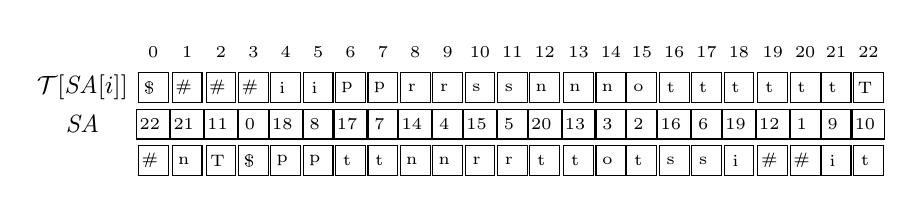
\begin{tikzpicture}

\matrix[
  matrix of nodes,
  row sep=2pt,
  nodes={
    draw,
    minimum height=2.5ex,
    minimum width=2.5ex,
    inner sep=1pt,
    font=\fontsize{6}{7}\selectfont,
    anchor=center,
    align=center
    }
  ]
 (mat) at (0,0)
 {
 \node[draw=none]{0}; & \node[draw=none]{1}; & \node[draw=none]{2}; & \node[draw=none]{3}; & \node[draw=none]{4}; & \node[draw=none]{5}; & 
 \node[draw=none]{6}; & \node[draw=none]{7}; & \node[draw=none]{8}; & \node[draw=none]{9}; & \node[draw=none]{10}; & \node[draw=none]{11}; &
 \node[draw=none]{12}; & \node[draw=none]{13}; & \node[draw=none]{14}; & \node[draw=none]{15}; & \node[draw=none]{16}; & \node[draw=none]{17}; &
 \node[draw=none]{18}; & \node[draw=none]{19}; & \node[draw=none]{20}; & \node[draw=none]{21}; & \node[draw=none]{22}; \\
 \$ & \# & \# & \# & i & i & p & p & r & r & s & s & n & n & n & o & t & t & t & t & t & t & T \\
 22 & 21 & 11 & 0 & 18 & 8 & 17 & 7 & 14 & 4 & 15 & 5 & 20 & 13 & 3 & 2 & 16 & 6 & 19 & 12 & 1 & 9 & 10 \\
\# & n & T &\$ &p &p &t &t &n &n  &r &r &t &t &o &t &s &s &i  &\# &\# &i &t \\
 };

%\node[left of=mat-1-1,node distance=.9cm] {\small $i$};
\node[left of=mat-2-1,node distance=.9cm] {\small $\col[\SA[i]]$};
\node[left of=mat-3-1,node distance=.9cm] {\small \SA};
\node[left of=mat-4-1,node distance=.9cm] {\small \colbwt};
\end{tikzpicture}
\label{fig-sa-bwt}
\end{subfigure}
\vspace{-0.8cm}
\caption{Data structures for the sample text {\col=``\#the old night keeper 
keeps the keep in the town\# the night keeper keeps the keep in the night\#\$}'' with alphabet {\alphabet=\{the, old, night, keeper, keeps, keep, in, town, \#\}} and code words {\em \$=0000}, {\em \#=0001}, 
{\em i=in=001}, {\em p=keep=010}, {\em r=keeper=011}, {\em s=keeps=1000}, 
{\em o=old=101}, {\em t=the=110}, {\em n=night=1001} and {\em T=town=111}.}
\label{fig-example}
\end{figure*}

Let {\col} be a string of size {\collen} drawn from an alphabet {\alphabet} of
size {\alphabetsize}. Let {$\col[i..\collen-1]$} be a {\it suffix} of {\col}.
The {\it suffix tree}~\cite{w-swat73} of {\col} is the compact labeled
tree of $\collen+1$ leaves where the root to leaf paths correspond to all suffixes of {\col\$},
where \$ is a terminating symbol not in {\alphabet}. The {\it path-label}
of each node $v$ corresponds to the concatenation of edge labels from the
root node to $v$. The {\it node depth} of $v$ corresponds to the number
of ancestors in the tree, whereas the {\it string depth} corresponds to the
length of the path-label. Searching for a pattern {\pattern} of 
size {\plen} in {\col} translates to finding the {\it locus} node $v$ closest to
the root such that {\pattern} is a prefix of the path-label of $v$ in $\Order{\plen}$ time.
We refer to this approach as {\it forward search}.
Figure~\ref{fig-suffix-tree} shows a suffix tree over a sample text. 
A suffix tree requires $\Order{\collen}$ space 
and can be constructed in $\Order{\collen}$ time~\cite{u-algo95}. The children
of each node in the suffix tree are lexicographically ordered by their edge labels.
The $i$-th smallest suffix in {\col} corresponds to the path-label of the $i$-th 
leaf. The starting position of the suffix can be associated its corresponding
leaf in the tree as shown in Figure~\ref{fig-suffix-tree}. All 
occurrences of {\pattern} in {\col} can be retrieved by visiting all leaves
in the subtree of the locus of {\pattern}. For example, pattern ``the night'' occurs
at positions $12$ and $19$ in the sample text. We further refer the number of children
of a node $v$ as its {\it degree} and the number of leaves in the subtree rooted at $v$
as the {\it size} of $v$.

The {\it suffix array}~\cite{mm-jcomp93} of {\col} is an array $\SA[0\ldots \collen-1]$ such
that $\SA[i]$ corresponds to the starting position of the $i$-th smallest suffix
in {\col} or the $i$-th leaf in the suffix tree of {\col}. The suffix array requires
$\collen \log \collen$ bits of space and can also be constructed in $\Order{\collen}$ time~\cite{ksb-jacm06}.
Using only the suffix array and the text, pattern search can be performed using binary search
in $\Order{\plen \log \collen}$ time. For example, the pattern ``the night'' is found by performing
binary search using \SA\ and \col\ to determine $\SA[18,19]$, the interval in 
\SA\ corresponding the the suffixes in \col\ prefixed by the pattern.
In practice, suffix arrays use $4-8\collen$ bytes of space whereas the most efficient
suffix tree implementations require at least $20\collen$ bytes of space~\cite{k-spe99} which
are both much larger than {\col} and prohibit the use of these structures for all but
small data sets.

\paragraph{Compressed Suffix Structures}
\label{sec-css}

Reducing the space usage of suffix based index structure has recently become an 
active area of research. The space usage of a suffix array can be reduced 
significantly by utilizing the compressibility of text combined 
with succinct data structures. A {\it succinct} data structure provides the
same functionality as an equivalent uncompressed data structure, but requires
only space equivalent to the information-theoretic lower bound of the underlying
data. For simplicity, we focus on the {\it FM-Index} which emulates the
functionality of a suffix array over $\col$ using $\collen H_k(\col)+o(\collen \log \sigma)$
bits of space where $H_k$ refers to the $k$-th order entropy of the text~\cite{fmmn-talg07}.
In practice, the FM-Index of $\col$ uses roughly space equivalent to
the compressed representation of $\col$ using a standard compressor such as {\tt bzip2}.
For a more comprehensive overview on succinct text indexes, see the
excellent survey of~\newcite{fgnv-jea08}.

The FM-Index relies on the duality between the suffix array and the BWT~\cite{bw-dec94}, 
a permutation of the text such that $\colbwt[i] = \col[\SA[i]-1]$ (see Figure~\ref{fig-example}). Searching for
a pattern using the FM-Index is performed in reverse order by performing  
{\rankop$(\colbwt,i,c)$} operations $\Order{\plen}$ times. Here, {\rankop$(\colbwt,i,c)$}  
counts the number of times symbol $c$ occurs in $\colbwt[0\ldots i-1]$. 
This process is usually referred to as {\it backward search}. Let $\SA[l_i,r_i]$ be
the interval corresponding to the suffixes in \col\ matching \pattern$[i\ldots \plen-1]$.
By definition of the BWT, $\colbwt[l_i,r_i]$ corresponds to the symbols in \col\
preceding \pattern$[i\ldots \plen-1]$ in \col. Due to the lexicographical ordering
of all suffixes in \SA, the interval $\SA[l_{i-1},r_{i-1}]$ corresponding to all
occurrences of \pattern$[i-1\ldots \plen-1]$ can be determined by computing the rank
of all occurrences of $c=\pattern[i-1]$ in $\colbwt[l_i,r_i]$. Thus, we compute
\rankop$(\colbwt,l_i,c)$, the number of times symbol $c$ occurs before
$l_i$ and \rankop$(\colbwt,r_i+1,c)$, the number of occurrences of $c$ in $\colbwt[0,r_i]$.
To determine $\SA[l_{i-1},r_{i-1}]$, we additionally store the starting positions $C_{s}$
of all suffixes for each symbol $s$ in $\alphabet$ at a negligible cost 
of $\alphabetsize \log \collen$ bits.
Thus, the new interval is computed as $l_{i-1} = C_c + $\rankop$(\colbwt,l_i,c)$ 
and $r_{i-1} = C_c + $\rankop$(\colbwt,r_i+1,c)$.


The time and space complexity of the FM-index thus depends on the cost of storing
and pre-processing \colbwt\ to answer \rankop\ efficiently. A {\it wavelet tree}
can be used to answer \rankop\ over $\colbwt$ in $\Order{\log \alphabetsize}$ time.
The wavelet tree reduces \rankop\ over an alphabet $\alphabet$ into multiple
\rankop\ operations over a binary alphabet which can be answered 
in $\Order{1}$ time and $o(\collen)$ bits extra space by periodically storing absolute
and relative \rankop\ counts~\cite{m-fsttcs96}. The alphabet is
reduced by recursively splitting symbols based on their code words into subgroups to 
form a binary tree as shown in Figure~\ref{fig-wt-bwt} for $\colbwt$. To answer
\rankop$(\colbwt,i,c)$, the tree is traversed based on the code word of $c$, performing
binary \rankop\ at each level. For example, \rankop$(\colbwt,17,\text{`t'})$ translates
to performing \rankop$(WT_{root},17,1)=12$ on the top level of the wavelet 
tree, as {\tt t=the=110}. We recurse to the right subtree of the root node and
compute \rankop$(WT_{1},12,1)$ as there were $12$ ones in the root node and
the next bit in the codeword of `the' is also one. This process continues until 
the correct leaf node is reached to answer \rankop$(\colbwt,17,\text{`t'})=5$ in 
$\Order{\log \alphabetsize}$ time. The space usage of a regular wavelet tree is
$\collen \log \alphabetsize + o(\collen \log \alphabetsize)$ bits which roughly
matches the size of the text.\footnote{However, if code-words for each symbol are chosen
based on their Huffman-codes the size of the wavelet tree reduces to $nH_0(\col)(1 + o(1))$
bits which can be further be reduced to to $\collen H_k(\col)+o(\collen \log \sigma)$ bits by using 
entropy compressed bitvectors.} If locations of matches are required, additional space is needed 
to access $\SA[i]$ or the inverse suffix array $\SA^{-1}[SA[i]]=i$. In the simplest scheme, both 
values are periodically sampled using a given sample rate \SASAMPLE (e.g. 32) such that $\SA[i] \mod \SASAMPLE = 0$. Then, 
for any $\SA[i]$ or $\SA^{-1}[i]$, at most $\Order{\SASAMPLE}$ \rankop\
operations on \colbwt\ are required to access the value.
Different sample rates, bitvector implementations and wavelet tree types result
in a wide variety of time-space tradeoffs which can be explored 
in practice~\cite{gbmp2014sea}.

In the same way the FM-index emulates the functionality of the suffix array in
little space, {\it compressed suffix trees} (\CST) provide the functionality
of suffix trees while requiring significantly less space than their uncompressed
counterparts~\cite{ofg-spire10}. A \CST uses a compressed suffix array (\CSA) such
as the FM-Index but stores additional information to represent the shape of
the suffix tree as well as information about path-labels. Again a variety
of different storage schemes exist, however for simplicity we focus on
the \CST of~\newcite{ofg-spire10} which we use in our experiments. Here, the 
shape of the tree is stored using a balanced-parenthesis (BP) sequence which 
for a tree of $p$ nodes requires $\approx 2p$ bits. Using little extra space
and advanced bit-operations, the BP-sequence can be used to perform 
operations such as \depth{}{$v$}, \parent{}{$v$} or 
accessing the $i$-th leaf can be answered in constant time.
To support more advanced operations such as accessing path-labels,
the underlying \CSA or a compressed version of the LCP array are required
which can be more expensive.\footnote{See \supp for an overview of the complexities
of the functionality of the \CST that is used in our experiments.} 
In practice, a \CST requires roughly $4-6\collen$ bits in addition to the
cost of storing the \CSA. For a more extensive overview of \CSTs see~\newcite{rno-talg11}.
%%% Local Variables: 
%%% mode: latex
%%% TeX-master: "cstlm"
%%% End: 


%\section{Language Modelling}
%\label{sec-lm}

\paragraph{Kneser Ney Language Modelling}
%\section{Kneser Ney Language Modelling}
\label{sec-lm}

%Background, mathematical formulation.

Recall our problem of efficient \ngram language modeling backed by a corpus encoded in a succinct index. % in such a way that they can be stored using only a small memory footprint and accessed efficiently. 
Although our method is generally applicable to many LM variants, we focus on the Kneser-Ney LM~\cite{kneser1995improved}, specifically the interpolated variant described in \newcite{chen1996empirical}, which has been shown to outperform other $n$gram LMs and has become the de-facto standard.

Interpolated Kneser-Ney describes the conditional probability of a word $w_i$ conditioned on the context of $m-1$ preceding words, $w_{i-m+1}^{i-1}$, as 
\begin{align}
P(w_i |& w_{i-m+1}^{i-1})=\frac{\max\left[c(w^{i}_{i-m+1}) - D_m,0\right]}{c(w^{i-1}_{i-m+1})} \nonumber \\
& \hspace{-6mm} +\frac{D_m \nlplus{w^{i-1}_{i-m-1}\Bigcdot} }{c(w^{i-1}_{i-m+1})}  
\bar{P}(w_i | w_{i-m+2}^{i-1}) ,  
\label{eq:high}
\end{align}
where lower-order smoothed probabilities are defined recursively (for $1<k<m$) as 
\begin{align}
\! \bar{P}(w_i |& w_{i-k+1}^{i-1})
 = \frac{\max\left[\nlplus{\Bigcdot w_{i-k+1}^{i}} - D_k,0\right]}{\nlplus{\Bigcdot w_{i-k+1}^{i-1} \Bigcdot}} \nonumber \\
&+ \frac{D_k \nlplus{w_{i-k+1}^{i-1}\Bigcdot}}{\nlplus{\Bigcdot w_{i-k+1}^{i-1} \Bigcdot}} \bar{P}(w_i | w_{i-k+2}^{i-1}) \,  . \! \label{eq:mid}
\end{align}
In the above formula, $D_k$ is the $k$gram-specific discount parameter, and 
the \emph{occurrence count} 
\mbox{$\nlplus{\alpha\Bigcdot} = |\{w: c(\alpha w)>0\}|$} 
is the number of observed word types following the pattern $\alpha$; 
the occurrence counts $\nlplus{\Bigcdot\alpha}$ and $\nlplus{\Bigcdot\alpha\Bigcdot}$ 
are defined accordingly.
%The highest order probability estimate in (\ref{eq:high}) interpolates a discounted frequency estimate with a $m-1$ order probability, defined as 
%Note the difference between (\ref{eq:mid})~and~(\ref{eq:high}), in that the frequency counts are redefined as occurrence counts. 
%The above equation is self-recursive, where each step shrinks the conditioning context by the least recent symbol. 
The recursion stops at unigram level where the unigram probabilities are defined as
%\begin{align*}
%\label{eq:low}
%
$ \bar{P}(w_i) = \nlplus{\Bigcdot w_i} / \nlplus{\Bigcdot\Bigcdot}$.%
\footnote{Modified Kneser-Ney, proposed
  by~\newcite{chen1996empirical}, typically outperforms interpolated
  Kneser-Ney through its use of context-specific discount parameters.
The implementation of this with our data structures is straightforward in principle, but brings a few added complexities in terms of dynamic computing other types of occurrence counts, which we leave for future work.}


%%% Local Variables: 
%%% mode: latex
%%% TeX-master: "cstlm"
%%% End: 


\section{Using \CSTs for KN Computation}
\label{sec-lmsdsl}
%Computing counts, N1+ of several flavours of different sized n-grams.

The key requirements for computing probability under a Kneser-Ney language model are two types of counts: raw frequencies of \ngrams and occurrence counts, quantifying how many different contexts the \ngram has occurred.
Figure~\ref{fig-counts-example} (right) illustrates the numbers needed in calculating the probability of an example 4-gram.
In electing to store the corpus directly in a suffix tree, we need to provide mechanisms for computing these counts based on queries into the suffix tree.

\begin{figure*}[tpb]
\centering
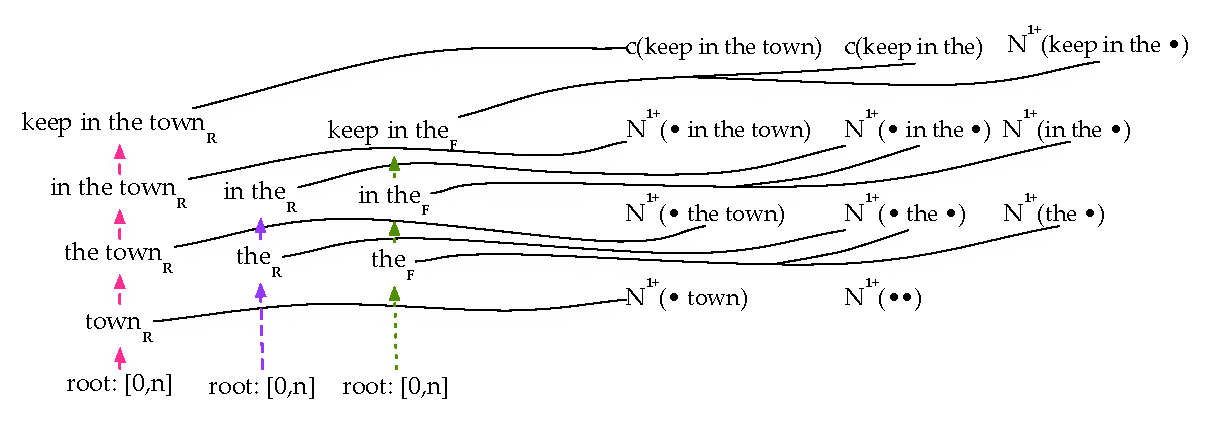
\includegraphics[width=0.85\textwidth]{figures/kn_dual_cst}
\vspace{-3ex}
\caption{Counts required for computing $P(\text{town} | \text{keep in the})$ (right) and the suffix tree nodes required for computing each value (left). The two left-most columns correspond to $\nrfull$ and $\nr$ and are updated using \emph{forward-search} in the reverse \CST, while the righter-most column correspond to $\nf$ and is updated using \emph{backward-search} in the forward \CST. See Algorithm~\ref{alg:pkn} for details.}
\label{fig-counts-example}
\end{figure*}


The raw frequency counts are the simplest to compute. First we
identify the locus node $v$ in the suffix tree for the query
\ngram; the frequency corresponds to the node's \emph{size}, an $\Order{1}$ 
operation which returns the number of descendents of $v$. To illustrate, consider
searching for \emph{the night} in  Figure~\ref{fig-suffix-tree}, which
matches a node with two descendents (labelled 19 and 12), and thus the
\ngram has count 2. 

More problematic are the occurrence counts, which come in several
flavours: with the dot to the right of the pattern, $\nlplus{\patdot}$,
to the left,  $\nlplus{\dotpat}$, and on both sides
$\nlplus{\dotpatdot}$. 
The first of these can be handled easily, as 
\begin{equation*}
\nlplus{\patdot} = \left\{ 
\begin{array}{ll}
   \degree{t}{v}, \quad & \text{if~} \alpha = \pathlabel{t}{v} \\
   1, & \text{otherwise}
\end{array} \right.
\end{equation*}
where $t$ is the \CST, $v$ is the node matching $\alpha$, and 
$\pathlabel{t}{v}$ denotes the label of the path from the root to $v$.%
\footnote{See the \supp for the explicit algorithm, but note there are some corner cases involving sentinels \#
  and \$, which shouldn't be counted when computing occurrence counts.
  Such tests have been omitted from the presentation for clarity. On publication the
  source code will be released with the complete implementation (roughly 1000 lines of C++).}
For example, \emph{keep in} has two child nodes in  Figure~\ref{fig-suffix-tree},
and thus there are two unique contexts in which it can occur, $\nlplus{\emph{keep in~}\Bigcdot}=2$,
while \emph{the keep} partially matches an edge in the forward suffix tree in
Figure~\ref{fig-suffix-tree} as it can only be followed by \emph{in}, $\nlplus{\emph{the keep~}\Bigcdot}=1$.
% This follows naturally from the suffix tree construction, where all descendent nodes correspond to larger \ngrams with same prefix, and each child edge extends the \ngram with a different subsequent symbol. 
% This method is illustrated in Algorithm~\ref{alg-nlplus}, which computes $\nlplus{\dotpat}$ 
% when $t$ is the reversed \CST and $\nlplus{\patdot}$ when $t$ is the forward \CST.
A similar line of reasoning applies to computing $\nlplus{\dotpat}$. 
Assuming we also have a second suffix tree representing the \emph{reversed corpus}, we first identify the reversed pattern (e.g., \emph{in keep}$_R$) and then use above method to compute the occurrence count (denoted hereafter $\nlplusfunc{t}{v}{\alpha}$). 

The final component of the Kneser-Ney LM computation is
$\nlplus{\dotpatdot}$, the number of unique contexts consider symbols
on both sides of the pattern. 
Unfortunately this does not map to a simple suffix tree operation,
but instead requires enumeration,
$\nlplus{\dotpatdot} = \sum_{s \in F(\alpha)} \nlplus{\dotpat s}$, 
where $F(\alpha)$ is the set of symbols that can follow $\alpha$.
%\end{equation*}
Algorithm~\ref{alg-occ-two-sided} shows how this is computed, with lines 7 and 8 enumerating $s \in F(\alpha)$ using the \emph{edge} labels of the children of $v$.
For each symbol, line 9 searches for an extended pattern incorporating the new symbol $s$ in the reverse \CSA (part of the reverse \CST), by refining the existing match $\nr$ using a single backward search operation after which we can compute $\nlplus{\patdot s}$.\footnote{Backward search in the reverse tree corresponds to extending the patttern to the right.}
% Finally we can query the unique left contexts for the node (line 10),
% which we accumulate to yield the return value.
Line 5 deals with the special case where the pattern does not match a complete edge, in which case there is only only unique right context and therefore $\nlplus{\dotpatdot} = \nlplus{\dotpat}$.

\begin{algorithm}[t]
  \caption{Two-sided occ., $\nlplus{\dotpatdot}$ 
    \label{alg:n1plusfb}}
\footnotesize
  \begin{algorithmic}[1]
    \Require{$\nf$ in forward \CST $\tf$ matches $\alpha$}
    \Require{$\nf$ in reverse \CST $\tr$ matches $\alpha$}
    \Function{N1PlusFrontBack}{$\tf, \nf, \tr, \nr, \alpha$} 
        \Let{$o$}{$0$}
        %\If{$\leaf{\tf}{\nf} \, \vee \, \depth{\tf}{\nf} > |\alpha|$}   \Comment{leaves and patterns internal to an edge}
        \Let{$d$}{$\depth{\tf}{\nf}$}   
        \If{$d > |\alpha|$}   %\Comment{patterns internal to an edge}
          \Let{$o$}{$\nlplusfunc{\tr}{\nr}{\dotpat}$} %\Comment{have only one right context}
        \Else
           \For{$\chf \gets \children{\tf}{\nf}$} 
              \Let{$s$}{$\edge{\tf}{\chf}{d+1}$} %\Comment{find the first symbol on the edge label}
              \Let{$\chr$}{$\backwardsearchnode{\tr}{\nr}{s}$} %\Comment{find child node in reverse \CST}
%              \Statex    %\Comment{$\ar$ is the \CSA component of $\tr$}
              \Let{$o$}{$o + \nlplusfunc{\tr}{\chr}{\dotpat s}$}
            \EndFor
        \EndIf
      \State \Return{$o$}
    \EndFunction
  \end{algorithmic}
\label{alg-occ-two-sided}
\end{algorithm}

\nlplusname and \nlplusfrontbackname can compute the requisite occurence counts for \ngram language modelling, however at considerable cost in terms of space and time. 
The need for twin reverse and forward \CSTs incurs a significant storage overhead, as well as the search time to match the pattern in both \CSTs. 
We show in Section \ref{sec-single-cst}  how we can avoid the need for the reversed suffix  tree, giving rise to lower memory requirements and faster runtime. 
Beyond the need for twin suffix trees, the highest time complexity calls are \emph{string-depth}, \emph{edge} and \emph{backward-search}.
Calling \emph{string-depth} is constant time for internal nodes, but $\Order{n\log\sigma}$ for leaf nodes; fortunately we can avoid this call for leaves, which by definition extend to the end of the corpus and consequently extend further than our pattern.\footnote{We assume search patterns do not extend beyond a single sentence, and thus will always be shorter than the edge labels.}
The costly calls to \emph{edge} and \emph{backward-search} however cannot be avoided.
This leads to an overall time complexity of $\Order{1}$ for \nlplusname and $\Order{F m \log\sigma}$ for \nlplusfrontbackname, where $F$ is the number of following symbols, $\sigma=|\Sigma|$ the vocabulary size, and $m=|\alpha|$ is the pattern length.

\section{Dual \CST Algorithm} 
\label{sec-dual-cst}

Using the methods above for computing the frequency and occurrence
counts, we now have the ingredients necessary to compute \ngram language model
probabilities. This leaves the algorithmic problem of efficiently ordering the search 
operations in forward and reverse \CST structures.

This paper considers an interpolated LM formulation, in which
probabilities from higher order contexts are interpolated with lower
order estimates.
% Our approach starts by querying the target word unigram $w_k$ and
% empty context $\emptyset$, from which the unigram probability can be computed
% Both patterns are extended to the left with symbol $w_{k-1}$, to form
% a bigram and the context unigram.
% In each step the probability is computed before extending the pattern,
% stopping after a fixed number of steps, $n$, or on encountering an
% unseen context.
This iterative process is apparent in Figure~\ref{fig-counts-example} (right) which shows the quantities required for probability scoring for an example \ngram.
Equivalently, the iteration can be considered in reverse, starting from unigram estimates and successively growing to large \ngrams, in each stage adding a single new symbol to left of the pattern. 
This suits incremental search in a \CST in which search bounds are iteratively refined, which has a substantially lower time complexity compared to searching over the full range.
%This fits well with cheaply searching a \CST one symbol at a time.  


\begin{algorithm}[tpb]
  \caption{KN probability $P\big(w_k | w^{k-1}_{k-(n-1)}\big)$
    \label{alg:pkn}}
\footnotesize
  \begin{algorithmic}[1]
    \Function{ProbKneserNey}{$\tf, \tr, \ws, n$} 
        \Let{$\nf$}{$\rooot{\tf}$} \Comment{match for context $w^{k-1}_{k-i}$}
        \Let{$\nr$}{$\rooot{\tr}$} \Comment{match for context $w^{k-1}_{k-i}$}
        \Let{$\nrfull$}{$\rooot{\tr}$} \Comment{match for $w^{k}_{k-i}$}
        \Let{$p$}{$1$}
        \For{$i \gets 1 \text{ to } $}
          \Let{$\nrfull$}{$\forwardsearchnode{\tr}{\nrfull}{w_{k-i+1}}$} %\Comment{update matches in \textsc{Cst}s}
          \If{$i > 1$}
             \Let{$\nf$}{$\backwardsearchnode{\tf}{\nf}{w_{k-i+1}}$} %\Comment{update context match in fwd \CST}
              \If{$i < m$}
             \Let{$\nr$}{$\forwardsearchnode{\tr}{\nr}{w_{k-i+1}}$} %\Comment{update context match in rev \CST}
          \EndIf
          \EndIf
          \Let{$D$}{lookup discount for $i$gram}
          \If{$i = m$} % or if s == '<s>' 
%                 \Comment{compute frequency count and denominator}
             \Let{$c$}{$\size{\tr}{\nrfull}$} 
             \Let{$d$}{$\size{\tf}{\nf}$}
          \Else  %\Comment{compute occurrence count and denominator}
             \Let{$c$}{$\nlplusfunc{\tr}{\nrfull}{\Bigcdot w^{k}_{k-i+1}}$} 
             \Let{$d$}{}
             \Statex \hfill $\nlplusfrontbackfunc{\tf}{\nf}{\nr}{\Bigcdot w^{k-1}_{k-i+1} \Bigcdot}$ %\Comment{precompute $\nlplus{\Bigcdot\Bigcdot}$}
           \EndIf
           \If{$i > 1$}
             \If{$\nf$ is valid} %\Comment{compute backoff probability, or backoff for unseen contexts}
                  \Let{$q$}{$\nlplusfunc{\tf}{\nf}{w^{k-1}_{k-i+1} \Bigcdot}$}  %\Comment{defined as $0$ for $i=1$}
                  \Let{$p$}{ $\frac{1}{d} \left( \max(c-D, 0)  + D  q  p \right)$} 
               \EndIf
          \ElsIf{$i = 1$}
              \Let{$p$}{$c  / \nlplus{\Bigcdot\Bigcdot}$}
          \EndIf
        \EndFor
      \State \Return{$p$}
    \EndFunction
  \end{algorithmic}
\label{alg-kn-slow}
\end{algorithm}



%\afterpage{\clearpage}

Algorithm~\ref{alg-kn-slow} presents an outline of the approach.
This uses a forward \CST, $\tf$, and a reverse \CST, $\tr$, with three \CST nodes (lines 2--4) tracking the match progress for the full $i$gram ($\nrfull$) and the $(i-1)$gram context ($\nf, \nr$), $i=1 \ldots m$.
The need to maintain three concurrent searches arises from the calls to size, $\nlplus{\dotpat}$, $\nlplus{\patdot}$ and $\nlplus{\dotpatdot}$ (lines 14, 15; 17; 21; and 18, respectively).
These calls impose conditions on the direction of the suffix tree, e.g., such that the edge 
labels and node degree can be used to compute the number of left or right contexts in which a pattern appears. 
The matching process is illustrated in Figure~\ref{fig-counts-example} where the three search nodes are shown on the left, considered bottom to top, and their corresponding count operations are shown to the right.
The $\nlplus{\dotpat}$ calls require a match in the reverse \CST (left-most column, $\nrfull$), while the $\nlplus{\patdot}$ require a match in the forward \CST (right-most column, $\nf$, matching the $(i-1)$gram context). 
The $\nlplus{\dotpatdot}$ computation reuses the forward match while also requiring a match for the $(i-1)$gram context in the reversed \CST, as tracked by the middle column ($\nr$).
Because of the mix of forward and reverse \CSTs, coupled with search patterns that are revealed right-to-left, incremental search in each of the \CSTs needs to be handled differently (lines 7--11).
In the forward \CST, we perform \emph{backward search} to extend the search pattern to the left, which can be computed very efficiently from the BWT in the \CSA.\footnote{See \supp Table~1 for the time complexities of this and other \CSA and \CST methods.}
Conversely in the reverse \CST, we must use \emph{forward search} as we are effectively extending the reversed pattern to the right; this operation is considerably more costly.

The discounts $D$ on line 12 of Algorithm~\ref{alg-kn-slow} and $\nlplus{\Bigcdot\Bigcdot}$ (line 18) are precomputed directly from the \CSTs thus avoiding several costly computations at runtime. 
The full algorithm is provided in Algorithm~8 in the \supp, which operates by traversing the nodes of the reverse \CST and at each stage computing the number of \ngrams that occur 1--4 times and $\nlplus{\dotpat}$ equal to 1--4, for various lengths of \ngrams.
These quantities are used to compute the discount parameters, which are then stored for use in estimation.\footnote{Discounts are computed up to a limit on \ngram size, here set to 10. The highest order values are used for computing the discount of \ngrams above the limit at runtime.}
Note that the \textsc{PrecomputeDiscounts} algorithm can be slow, although it is significantly faster if we remove the \emph{edge} calls and simply include in our counts all \ngrams finishing a sentence or spanning more than one sentence. 
These approximate discounts are typically within $10^{-2}$ of the correct values.

\section{Improved Single \CST Approach}
\label{sec-single-cst}

The above dual \CST algorithm provides an elegant means of computing LM probabilities of arbitrary order and with a limited space complexity ($\Order{n}$, or roughly $n$ in practice).
However the time complexity is problematic, stemming from the expensive method for computing \nlplusfrontbackname and repeated searches over the \CST, particularly \emph{forward-search}.
Now we outline a method for speeding up the algorithm by doing away with the reverse \CST.
Instead the critical counts, $\nlplus{\dotpat}$ and $\nlplus{\dotpatdot}$ are computed directly from a single forward \CST. 
This confers the benefit of using only backward search and avoiding redundant searches for the same pattern (cf.~lines 9 and 11 in Alg~\ref{alg-kn-slow}).


The full algorithm for computing LM probabilities is given in the \supp as Algorithm 7, however for space reasons we will not describe this in detail.
Instead we will focus on the method's most critical component, the algorithm for computing $\nlplus{\dotpatdot}$ from the forward \CST, presented in Alg~\ref{alg:n1plusfb_wt}.
The key different from Alg~\ref{alg:n1plusfb} is the loop from lines 6--9, which uses the \emph{interval-symbols} method.
This method assumes a \emph{wavelet tree} representation of the \SA component of the \CST, an efficient encoding of the \emph{Burrows-Wheeler transform} (an array comprising the symbol preceeding each entry in the \SA).
The \emph{interval-symbols} method uses rank and select bit operations to efficiently identify for a given pattern the set of preceeding symbols, and for each of symbol the range of occurrences this corresponds to in the \SA.
For example, in Figure~\ref{fig-suffix-tree} the pattern $\alpha=\text{``night''}$ is preceeded by $s=$``old'' and $s=$``the''.
These correspond to the only occurrence of ``old'', and the 4$^{th}$ and 5$^{th}$ occurrence of ``the'' in the BWT.
These occurence bounds can then be used to calculate the range in the \SA by adding to $C_s$, the precomputed offset of the first pattern beginning with $s$, exploiting the property that the \SA is lexicographically sorted.
In the example above, $C_{\text{the}} = 16$ (``the'' corresponds to \SA entries 16--20) and therefore the location of ``the night'' is therefore $[16+(4-1),16+(5-1)] = [19,20]$ (the $-1$ adjusts for counting from 1 in the above exposition, rather than 0).


\begin{algorithm}[t]
  \caption{%Two-sided occ, 
$\nlplus{\dotpatdot}$, using forward \CST 
    \label{alg:n1plusfb_wt}}
\footnotesize
  \begin{algorithmic}[1]
    \Require{$\nf$ in forward \CST $\tf$ matches $\alpha$}
%    \Require{the \CSA component, $\af$ of $\tf$ is a wavelet tree}
    \Function{\nlplusfrontbacklname}{$\tf, \nf, \alpha$} 
        \Let{$o$}{$0$}
        %\If{$\leaf{\tf}{\nf} \, \vee \, \depth{\tf}{\nf} > |\alpha|$}   
        \If{$\depth{\tf}{\nf} > |\alpha|$}   
          \Let{$o$}{$\nlplusbacklfunc{\tf}{\nf}{\dotpat}$} %\Comment{only one unique right context}
        \Else
            \For{$\langle l, r, s\rangle \gets \intervalsymbols{\tf}{\lb{\nf}}{\rb{\nf}}$}
               \Let{$l'$}{$C_s + l$}% \Comment{compute offsets into \SA for patterns starting with symbol $s$}
               \Let{$r'$}{$C_s + r$} %\Comment{adjusted by occurence indices $[l,r]$}
               \Let{$o$}{$o + \nlplusbacklfunc{\tf}{\text{node}(l', r')}{\dotpat s}$}
            \EndFor
          \EndIf
      \State \Return{$o$}
    \EndFunction
  \end{algorithmic}
\end{algorithm}

\nlplusbacklname is computed in a similar way, using the \emph{interval-symbols} method to compute the number of unique preceeding symbols (see \supp, Algorithm~6).
Overall the time complexity of inference for both \nlplusbacklname and \nlplusfrontbacklname is $\Order{k \log \sigma}$ where $k$ is the number of preceeding symbols, a considerable improvement over \nlplusfrontbackname using the forward and reverse \CSTs.
Overall this leads to considerably faster computation of \ngram probabilities compared to the two \CST approach, and although still slower than highly optimised LM toolkits like \textsc{Srilm}, it is fast enough to support large scale experiments, and has considerably better scaling performance with the Markov order $m$ (even allowing unlimited order), as we will now demonstrate.


%%% Local Variables: 
%%% mode: latex
%%% TeX-master: "cstlm"
%%% End: 


\section{Experiments}
\label{sec-experiments}

\subsection{Datasets}
We used Europarl dataset and the data was numberized after tokenizing, splitting, and excluding xml markups. The first $10K$ sentences were used as the test data, and the last 80\% as the training data (See Table~\ref{fig:data}).

\begin{table}
\resizebox{1\columnwidth}{!}{
\begin{tabular}{ll|cc|c}
Language&&Size (MB)&Tokens (M)& Sentences (K)\\
\toprule 
Bulgarian&BG&36.11&8.53&329\\
Czech&CS&53.48&12.25&535\\
German&DE&171.80&44.07&1785 \\
English&EN&179.15&49.32&1815\\
Finnish&FI&145.32&32.85&1737\\
French&FR&197.68&53.82&1792\\
Hungarian&HU&52.53&12.02&527\\
Italian&IT&186.67&48.08&1703\\
Portuguese&PT&187.20&49.03&1737\\
\end{tabular}}
\caption{Tokens and sentence counts refer to the training partition. \trevor{Move to \supp}}\label{fig:data}
\end{table}
Figure~\ref{fig:data} is showing XXX.
\begin{figure}
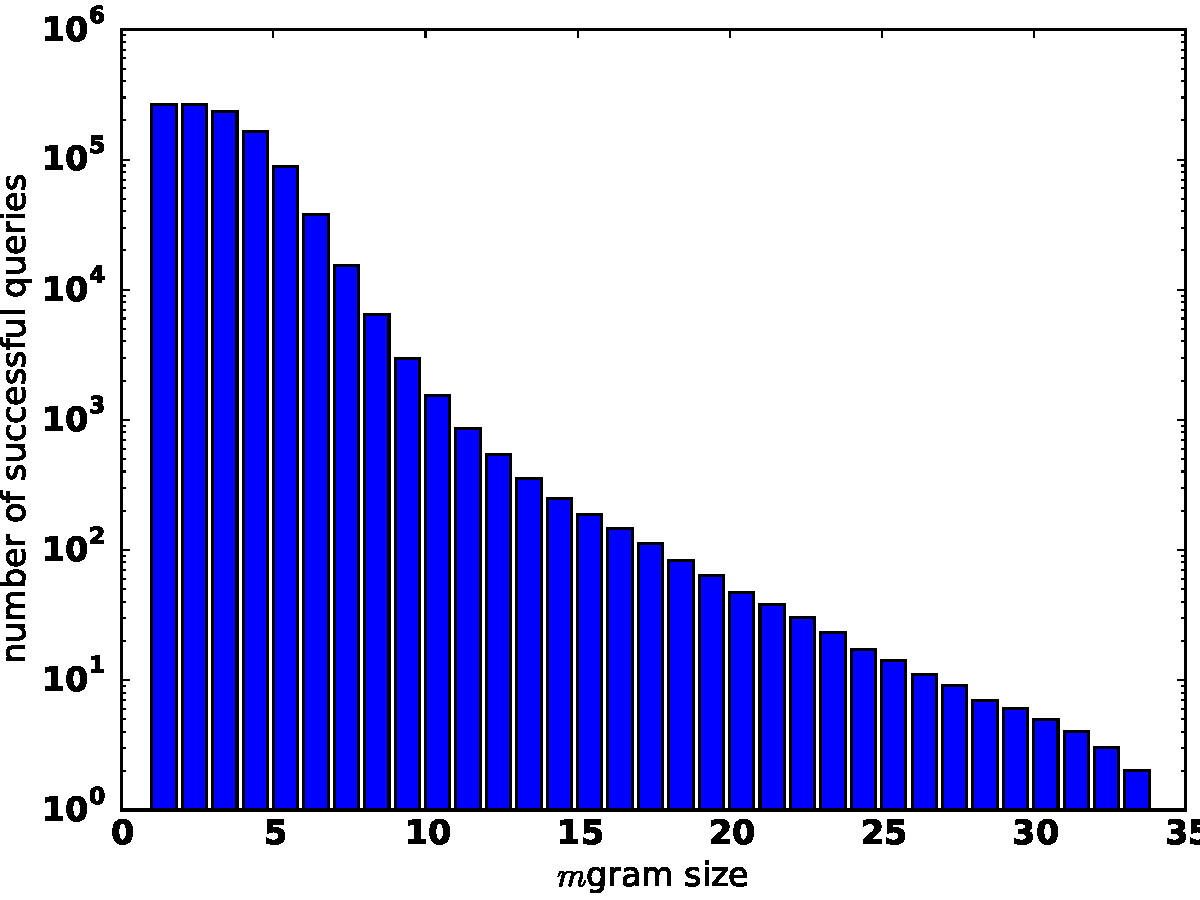
\includegraphics[width=\columnwidth]{figures/german_pattern_size.pdf}
\caption{Number of successful queries across different pattern sizes from KN computation over the German test set, with unbounded $m$.}
\end{figure}\label{fig:germanpattern}

\subsection{Perplexity Evaluation}
We evaluated the perplexity across different languages and using different order $m$-grams varying from $2$ to $\infty=99999$. While matching SRILM in perplexity we compared our time and memory usage during the training and query time. Figure~\ref{figure:pplx} shows the gain in perplexity with respect to $m$. 
\begin{figure}
% Created by tikzDevice version 0.8.1 on 2015-05-31 13:53:07
% !TEX encoding = UTF-8 Unicode
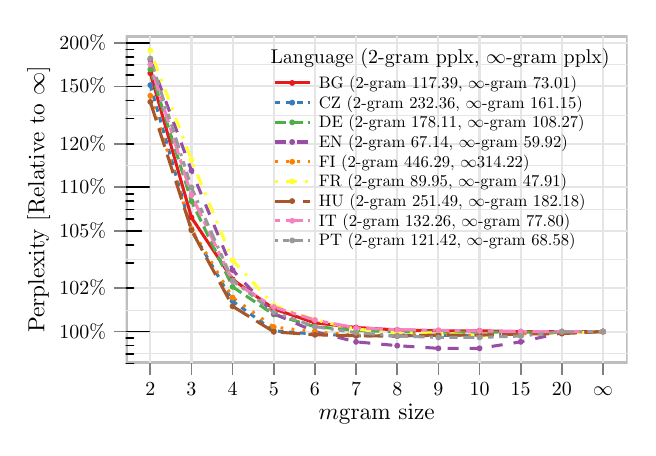
\begin{tikzpicture}[x=1pt,y=1pt]
\definecolor{fillColor}{RGB}{255,255,255}
\path[use as bounding box,fill=fillColor,fill opacity=0.00] (0,0) rectangle (216.81,144.54);
\begin{scope}
\path[clip] (  0.00,  0.00) rectangle (216.81,144.54);
\definecolor{fillColor}{RGB}{255,255,255}

\path[fill=fillColor] (  0.00,  0.00) rectangle (216.81,144.54);
\end{scope}
\begin{scope}
\path[clip] ( 35.40, 23.29) rectangle (216.81,141.69);
\definecolor{drawColor}{RGB}{190,190,190}

\path[draw=drawColor,line width= 1.5pt,line join=round,line cap=round] ( 35.40, 23.29) rectangle (216.81,141.69);
\definecolor{drawColor}{gray}{0.90}

\path[draw=drawColor,line width= 0.3pt,line join=round] ( 35.40, 26.85) --
	(216.81, 26.85);

\path[draw=drawColor,line width= 0.3pt,line join=round] ( 35.40, 42.55) --
	(216.81, 42.55);

\path[draw=drawColor,line width= 0.3pt,line join=round] ( 35.40, 60.78) --
	(216.81, 60.78);

\path[draw=drawColor,line width= 0.3pt,line join=round] ( 35.40, 79.01) --
	(216.81, 79.01);

\path[draw=drawColor,line width= 0.3pt,line join=round] ( 35.40, 94.71) --
	(216.81, 94.71);

\path[draw=drawColor,line width= 0.3pt,line join=round] ( 35.40,112.94) --
	(216.81,112.94);

\path[draw=drawColor,line width= 0.3pt,line join=round] ( 35.40,131.17) --
	(216.81,131.17);

\path[draw=drawColor,line width= 0.8pt,line join=round] ( 35.40, 34.70) --
	(216.81, 34.70);

\path[draw=drawColor,line width= 0.8pt,line join=round] ( 35.40, 50.40) --
	(216.81, 50.40);

\path[draw=drawColor,line width= 0.8pt,line join=round] ( 35.40, 71.16) --
	(216.81, 71.16);

\path[draw=drawColor,line width= 0.8pt,line join=round] ( 35.40, 86.86) --
	(216.81, 86.86);

\path[draw=drawColor,line width= 0.8pt,line join=round] ( 35.40,102.56) --
	(216.81,102.56);

\path[draw=drawColor,line width= 0.8pt,line join=round] ( 35.40,123.32) --
	(216.81,123.32);

\path[draw=drawColor,line width= 0.8pt,line join=round] ( 35.40,139.02) --
	(216.81,139.02);

\path[draw=drawColor,line width= 0.8pt,line join=round] ( 44.32, 23.29) --
	( 44.32,141.69);

\path[draw=drawColor,line width= 0.8pt,line join=round] ( 59.19, 23.29) --
	( 59.19,141.69);

\path[draw=drawColor,line width= 0.8pt,line join=round] ( 74.06, 23.29) --
	( 74.06,141.69);

\path[draw=drawColor,line width= 0.8pt,line join=round] ( 88.93, 23.29) --
	( 88.93,141.69);

\path[draw=drawColor,line width= 0.8pt,line join=round] (103.80, 23.29) --
	(103.80,141.69);

\path[draw=drawColor,line width= 0.8pt,line join=round] (118.67, 23.29) --
	(118.67,141.69);

\path[draw=drawColor,line width= 0.8pt,line join=round] (133.54, 23.29) --
	(133.54,141.69);

\path[draw=drawColor,line width= 0.8pt,line join=round] (148.41, 23.29) --
	(148.41,141.69);

\path[draw=drawColor,line width= 0.8pt,line join=round] (163.28, 23.29) --
	(163.28,141.69);

\path[draw=drawColor,line width= 0.8pt,line join=round] (178.15, 23.29) --
	(178.15,141.69);

\path[draw=drawColor,line width= 0.8pt,line join=round] (193.02, 23.29) --
	(193.02,141.69);

\path[draw=drawColor,line width= 0.8pt,line join=round] (207.89, 23.29) --
	(207.89,141.69);
\definecolor{drawColor}{RGB}{228,26,28}

\path[draw=drawColor,line width= 1.1pt,line join=round] ( 44.32,128.11) --
	( 59.19, 75.95) --
	( 74.06, 53.58) --
	( 88.93, 42.93) --
	(103.80, 37.88) --
	(118.67, 36.20) --
	(133.54, 35.31) --
	(148.41, 35.01) --
	(163.28, 35.01) --
	(178.15, 34.70) --
	(193.02, 34.70) --
	(207.89, 34.70);
\definecolor{drawColor}{RGB}{55,126,184}

\path[draw=drawColor,line width= 1.1pt,dash pattern=on 2pt off 2pt ,line join=round] ( 44.32,123.78) --
	( 59.19, 71.41) --
	( 74.06, 45.72) --
	( 88.93, 34.99) --
	(103.80, 33.81) --
	(118.67, 33.19) --
	(133.54, 33.19) --
	(148.41, 33.34) --
	(163.28, 33.34) --
	(178.15, 34.41) --
	(193.02, 34.55) --
	(207.89, 34.70);
\definecolor{drawColor}{RGB}{77,175,74}

\path[draw=drawColor,line width= 1.1pt,dash pattern=on 4pt off 2pt ,line join=round] ( 44.32,129.43) --
	( 59.19, 81.86) --
	( 74.06, 50.89) --
	( 88.93, 40.89) --
	(103.80, 36.51) --
	(118.67, 35.12) --
	(133.54, 34.70) --
	(148.41, 34.49) --
	(163.28, 34.49) --
	(178.15, 34.49) --
	(193.02, 34.70) --
	(207.89, 34.70);
\definecolor{drawColor}{RGB}{152,78,163}

\path[draw=drawColor,line width= 1.1pt,dash pattern=on 4pt off 4pt ,line join=round] ( 44.32,132.99) --
	( 59.19, 92.89) --
	( 74.06, 56.94) --
	( 88.93, 41.23) --
	(103.80, 34.70) --
	(118.67, 31.01) --
	(133.54, 29.64) --
	(148.41, 28.67) --
	(163.28, 28.67) --
	(178.15, 31.01) --
	(193.02, 34.32) --
	(207.89, 34.70);
\definecolor{drawColor}{RGB}{255,127,0}

\path[draw=drawColor,line width= 1.1pt,dash pattern=on 1pt off 3pt ,line join=round] ( 44.32,119.92) --
	( 59.19, 71.83) --
	( 74.06, 47.02) --
	( 88.93, 36.37) --
	(103.80, 34.63) --
	(118.67, 33.44) --
	(133.54, 33.52) --
	(148.41, 33.67) --
	(163.28, 33.29) --
	(178.15, 33.97) --
	(193.02, 34.48) --
	(207.89, 34.70);
\definecolor{drawColor}{RGB}{255,255,51}

\path[draw=drawColor,line width= 1.1pt,dash pattern=on 1pt off 3pt on 4pt off 3pt ,line join=round] ( 44.32,136.31) --
	( 59.19, 96.73) --
	( 74.06, 60.54) --
	( 88.93, 44.21) --
	(103.80, 38.99) --
	(118.67, 35.63) --
	(133.54, 34.22) --
	(148.41, 34.22) --
	(163.28, 33.24) --
	(178.15, 33.74) --
	(193.02, 34.22) --
	(207.89, 34.70);
\definecolor{drawColor}{RGB}{166,86,40}

\path[draw=drawColor,line width= 1.1pt,dash pattern=on 7pt off 3pt ,line join=round] ( 44.32,117.71) --
	( 59.19, 71.37) --
	( 74.06, 43.85) --
	( 88.93, 34.64) --
	(103.80, 33.55) --
	(118.67, 33.23) --
	(133.54, 33.12) --
	(148.41, 33.49) --
	(163.28, 33.45) --
	(178.15, 33.81) --
	(193.02, 33.99) --
	(207.89, 34.70);
\definecolor{drawColor}{RGB}{247,129,191}

\path[draw=drawColor,line width= 1.1pt,dash pattern=on 2pt off 2pt on 6pt off 2pt ,line join=round] ( 44.32,131.26) --
	( 59.19, 84.00) --
	( 74.06, 52.90) --
	( 88.93, 43.58) --
	(103.80, 38.87) --
	(118.67, 36.02) --
	(133.54, 35.40) --
	(148.41, 35.21) --
	(163.28, 34.95) --
	(178.15, 34.72) --
	(193.02, 34.69) --
	(207.89, 34.70);
\definecolor{drawColor}{gray}{0.60}

\path[draw=drawColor,line width= 1.1pt,dash pattern=on 1pt off 2pt on 2pt off 2pt on 3pt off 2pt on 4pt off 2pt ,line join=round] ( 44.32,133.40) --
	( 59.19, 86.79) --
	( 74.06, 53.23) --
	( 88.93, 41.73) --
	(103.80, 36.54) --
	(118.67, 34.31) --
	(133.54, 33.17) --
	(148.41, 32.59) --
	(163.28, 32.62) --
	(178.15, 33.11) --
	(193.02, 34.63) --
	(207.89, 34.70);
\definecolor{fillColor}{RGB}{228,26,28}

\path[fill=fillColor] ( 44.32,128.11) circle (  1.07);

\path[fill=fillColor] ( 59.19, 75.95) circle (  1.07);

\path[fill=fillColor] ( 74.06, 53.58) circle (  1.07);

\path[fill=fillColor] ( 88.93, 42.93) circle (  1.07);

\path[fill=fillColor] (103.80, 37.88) circle (  1.07);

\path[fill=fillColor] (118.67, 36.20) circle (  1.07);

\path[fill=fillColor] (133.54, 35.31) circle (  1.07);

\path[fill=fillColor] (148.41, 35.01) circle (  1.07);

\path[fill=fillColor] (163.28, 35.01) circle (  1.07);

\path[fill=fillColor] (178.15, 34.70) circle (  1.07);

\path[fill=fillColor] (193.02, 34.70) circle (  1.07);

\path[fill=fillColor] (207.89, 34.70) circle (  1.07);
\definecolor{fillColor}{RGB}{55,126,184}

\path[fill=fillColor] ( 44.32,123.78) circle (  1.07);

\path[fill=fillColor] ( 59.19, 71.41) circle (  1.07);

\path[fill=fillColor] ( 74.06, 45.72) circle (  1.07);

\path[fill=fillColor] ( 88.93, 34.99) circle (  1.07);

\path[fill=fillColor] (103.80, 33.81) circle (  1.07);

\path[fill=fillColor] (118.67, 33.19) circle (  1.07);

\path[fill=fillColor] (133.54, 33.19) circle (  1.07);

\path[fill=fillColor] (148.41, 33.34) circle (  1.07);

\path[fill=fillColor] (163.28, 33.34) circle (  1.07);

\path[fill=fillColor] (178.15, 34.41) circle (  1.07);

\path[fill=fillColor] (193.02, 34.55) circle (  1.07);

\path[fill=fillColor] (207.89, 34.70) circle (  1.07);
\definecolor{fillColor}{RGB}{77,175,74}

\path[fill=fillColor] ( 44.32,129.43) circle (  1.07);

\path[fill=fillColor] ( 59.19, 81.86) circle (  1.07);

\path[fill=fillColor] ( 74.06, 50.89) circle (  1.07);

\path[fill=fillColor] ( 88.93, 40.89) circle (  1.07);

\path[fill=fillColor] (103.80, 36.51) circle (  1.07);

\path[fill=fillColor] (118.67, 35.12) circle (  1.07);

\path[fill=fillColor] (133.54, 34.70) circle (  1.07);

\path[fill=fillColor] (148.41, 34.49) circle (  1.07);

\path[fill=fillColor] (163.28, 34.49) circle (  1.07);

\path[fill=fillColor] (178.15, 34.49) circle (  1.07);

\path[fill=fillColor] (193.02, 34.70) circle (  1.07);

\path[fill=fillColor] (207.89, 34.70) circle (  1.07);
\definecolor{fillColor}{RGB}{152,78,163}

\path[fill=fillColor] ( 44.32,132.99) circle (  1.07);

\path[fill=fillColor] ( 59.19, 92.89) circle (  1.07);

\path[fill=fillColor] ( 74.06, 56.94) circle (  1.07);

\path[fill=fillColor] ( 88.93, 41.23) circle (  1.07);

\path[fill=fillColor] (103.80, 34.70) circle (  1.07);

\path[fill=fillColor] (118.67, 31.01) circle (  1.07);

\path[fill=fillColor] (133.54, 29.64) circle (  1.07);

\path[fill=fillColor] (148.41, 28.67) circle (  1.07);

\path[fill=fillColor] (163.28, 28.67) circle (  1.07);

\path[fill=fillColor] (178.15, 31.01) circle (  1.07);

\path[fill=fillColor] (193.02, 34.32) circle (  1.07);

\path[fill=fillColor] (207.89, 34.70) circle (  1.07);
\definecolor{fillColor}{RGB}{255,127,0}

\path[fill=fillColor] ( 44.32,119.92) circle (  1.07);

\path[fill=fillColor] ( 59.19, 71.83) circle (  1.07);

\path[fill=fillColor] ( 74.06, 47.02) circle (  1.07);

\path[fill=fillColor] ( 88.93, 36.37) circle (  1.07);

\path[fill=fillColor] (103.80, 34.63) circle (  1.07);

\path[fill=fillColor] (118.67, 33.44) circle (  1.07);

\path[fill=fillColor] (133.54, 33.52) circle (  1.07);

\path[fill=fillColor] (148.41, 33.67) circle (  1.07);

\path[fill=fillColor] (163.28, 33.29) circle (  1.07);

\path[fill=fillColor] (178.15, 33.97) circle (  1.07);

\path[fill=fillColor] (193.02, 34.48) circle (  1.07);

\path[fill=fillColor] (207.89, 34.70) circle (  1.07);
\definecolor{fillColor}{RGB}{255,255,51}

\path[fill=fillColor] ( 44.32,136.31) circle (  1.07);

\path[fill=fillColor] ( 59.19, 96.73) circle (  1.07);

\path[fill=fillColor] ( 74.06, 60.54) circle (  1.07);

\path[fill=fillColor] ( 88.93, 44.21) circle (  1.07);

\path[fill=fillColor] (103.80, 38.99) circle (  1.07);

\path[fill=fillColor] (118.67, 35.63) circle (  1.07);

\path[fill=fillColor] (133.54, 34.22) circle (  1.07);

\path[fill=fillColor] (148.41, 34.22) circle (  1.07);

\path[fill=fillColor] (163.28, 33.24) circle (  1.07);

\path[fill=fillColor] (178.15, 33.74) circle (  1.07);

\path[fill=fillColor] (193.02, 34.22) circle (  1.07);

\path[fill=fillColor] (207.89, 34.70) circle (  1.07);
\definecolor{fillColor}{RGB}{166,86,40}

\path[fill=fillColor] ( 44.32,117.71) circle (  1.07);

\path[fill=fillColor] ( 59.19, 71.37) circle (  1.07);

\path[fill=fillColor] ( 74.06, 43.85) circle (  1.07);

\path[fill=fillColor] ( 88.93, 34.64) circle (  1.07);

\path[fill=fillColor] (103.80, 33.55) circle (  1.07);

\path[fill=fillColor] (118.67, 33.23) circle (  1.07);

\path[fill=fillColor] (133.54, 33.12) circle (  1.07);

\path[fill=fillColor] (148.41, 33.49) circle (  1.07);

\path[fill=fillColor] (163.28, 33.45) circle (  1.07);

\path[fill=fillColor] (178.15, 33.81) circle (  1.07);

\path[fill=fillColor] (193.02, 33.99) circle (  1.07);

\path[fill=fillColor] (207.89, 34.70) circle (  1.07);
\definecolor{fillColor}{RGB}{247,129,191}

\path[fill=fillColor] ( 44.32,131.26) circle (  1.07);

\path[fill=fillColor] ( 59.19, 84.00) circle (  1.07);

\path[fill=fillColor] ( 74.06, 52.90) circle (  1.07);

\path[fill=fillColor] ( 88.93, 43.58) circle (  1.07);

\path[fill=fillColor] (103.80, 38.87) circle (  1.07);

\path[fill=fillColor] (118.67, 36.02) circle (  1.07);

\path[fill=fillColor] (133.54, 35.40) circle (  1.07);

\path[fill=fillColor] (148.41, 35.21) circle (  1.07);

\path[fill=fillColor] (163.28, 34.95) circle (  1.07);

\path[fill=fillColor] (178.15, 34.72) circle (  1.07);

\path[fill=fillColor] (193.02, 34.69) circle (  1.07);

\path[fill=fillColor] (207.89, 34.70) circle (  1.07);
\definecolor{fillColor}{gray}{0.60}

\path[fill=fillColor] ( 44.32,133.40) circle (  1.07);

\path[fill=fillColor] ( 59.19, 86.79) circle (  1.07);

\path[fill=fillColor] ( 74.06, 53.23) circle (  1.07);

\path[fill=fillColor] ( 88.93, 41.73) circle (  1.07);

\path[fill=fillColor] (103.80, 36.54) circle (  1.07);

\path[fill=fillColor] (118.67, 34.31) circle (  1.07);

\path[fill=fillColor] (133.54, 33.17) circle (  1.07);

\path[fill=fillColor] (148.41, 32.59) circle (  1.07);

\path[fill=fillColor] (163.28, 32.62) circle (  1.07);

\path[fill=fillColor] (178.15, 33.11) circle (  1.07);

\path[fill=fillColor] (193.02, 34.63) circle (  1.07);

\path[fill=fillColor] (207.89, 34.70) circle (  1.07);
\definecolor{drawColor}{RGB}{0,0,0}

\path[draw=drawColor,line width= 0.6pt,line join=round,line cap=round] ( 35.40,  7.43) -- ( 38.25,  7.43);

\path[draw=drawColor,line width= 0.6pt,line join=round,line cap=round] ( 35.40, 13.95) -- ( 38.25, 13.95);

\path[draw=drawColor,line width= 0.6pt,line join=round,line cap=round] ( 35.40, 19.00) -- ( 41.09, 19.00);

\path[draw=drawColor,line width= 0.6pt,line join=round,line cap=round] ( 35.40, 23.13) -- ( 38.25, 23.13);

\path[draw=drawColor,line width= 0.6pt,line join=round,line cap=round] ( 35.40, 26.62) -- ( 38.25, 26.62);

\path[draw=drawColor,line width= 0.6pt,line join=round,line cap=round] ( 35.40, 29.65) -- ( 38.25, 29.65);

\path[draw=drawColor,line width= 0.6pt,line join=round,line cap=round] ( 35.40, 32.31) -- ( 38.25, 32.31);

\path[draw=drawColor,line width= 0.6pt,line join=round,line cap=round] ( 35.40, 34.70) -- ( 43.94, 34.70);

\path[draw=drawColor,line width= 0.6pt,line join=round,line cap=round] ( 35.40, 50.40) -- ( 38.25, 50.40);

\path[draw=drawColor,line width= 0.6pt,line join=round,line cap=round] ( 35.40, 59.59) -- ( 38.25, 59.59);

\path[draw=drawColor,line width= 0.6pt,line join=round,line cap=round] ( 35.40, 66.10) -- ( 38.25, 66.10);

\path[draw=drawColor,line width= 0.6pt,line join=round,line cap=round] ( 35.40, 71.16) -- ( 41.09, 71.16);

\path[draw=drawColor,line width= 0.6pt,line join=round,line cap=round] ( 35.40, 75.29) -- ( 38.25, 75.29);

\path[draw=drawColor,line width= 0.6pt,line join=round,line cap=round] ( 35.40, 78.78) -- ( 38.25, 78.78);

\path[draw=drawColor,line width= 0.6pt,line join=round,line cap=round] ( 35.40, 81.80) -- ( 38.25, 81.80);

\path[draw=drawColor,line width= 0.6pt,line join=round,line cap=round] ( 35.40, 84.47) -- ( 38.25, 84.47);

\path[draw=drawColor,line width= 0.6pt,line join=round,line cap=round] ( 35.40, 86.86) -- ( 43.94, 86.86);

\path[draw=drawColor,line width= 0.6pt,line join=round,line cap=round] ( 35.40,102.56) -- ( 38.25,102.56);

\path[draw=drawColor,line width= 0.6pt,line join=round,line cap=round] ( 35.40,111.74) -- ( 38.25,111.74);

\path[draw=drawColor,line width= 0.6pt,line join=round,line cap=round] ( 35.40,118.26) -- ( 38.25,118.26);

\path[draw=drawColor,line width= 0.6pt,line join=round,line cap=round] ( 35.40,123.32) -- ( 41.09,123.32);

\path[draw=drawColor,line width= 0.6pt,line join=round,line cap=round] ( 35.40,127.45) -- ( 38.25,127.45);

\path[draw=drawColor,line width= 0.6pt,line join=round,line cap=round] ( 35.40,130.94) -- ( 38.25,130.94);

\path[draw=drawColor,line width= 0.6pt,line join=round,line cap=round] ( 35.40,133.96) -- ( 38.25,133.96);

\path[draw=drawColor,line width= 0.6pt,line join=round,line cap=round] ( 35.40,136.63) -- ( 38.25,136.63);

\path[draw=drawColor,line width= 0.6pt,line join=round,line cap=round] ( 35.40,139.02) -- ( 43.94,139.02);
\end{scope}
\begin{scope}
\path[clip] (  0.00,  0.00) rectangle (216.81,144.54);
\definecolor{drawColor}{RGB}{0,0,0}

\node[text=drawColor,anchor=base east,inner sep=0pt, outer sep=0pt, scale=  0.72] at ( 28.29, 32.36) {100\%};

\node[text=drawColor,anchor=base east,inner sep=0pt, outer sep=0pt, scale=  0.72] at ( 28.29, 48.06) {102\%};

\node[text=drawColor,anchor=base east,inner sep=0pt, outer sep=0pt, scale=  0.72] at ( 28.29, 68.81) {105\%};

\node[text=drawColor,anchor=base east,inner sep=0pt, outer sep=0pt, scale=  0.72] at ( 28.29, 84.52) {110\%};

\node[text=drawColor,anchor=base east,inner sep=0pt, outer sep=0pt, scale=  0.72] at ( 28.29,100.22) {120\%};

\node[text=drawColor,anchor=base east,inner sep=0pt, outer sep=0pt, scale=  0.72] at ( 28.29,120.97) {150\%};

\node[text=drawColor,anchor=base east,inner sep=0pt, outer sep=0pt, scale=  0.72] at ( 28.29,136.67) {200\%};
\end{scope}
\begin{scope}
\path[clip] (  0.00,  0.00) rectangle (216.81,144.54);
\definecolor{drawColor}{gray}{0.50}

\path[draw=drawColor,line width= 0.6pt,line join=round] ( 31.13, 34.70) --
	( 35.40, 34.70);

\path[draw=drawColor,line width= 0.6pt,line join=round] ( 31.13, 50.40) --
	( 35.40, 50.40);

\path[draw=drawColor,line width= 0.6pt,line join=round] ( 31.13, 71.16) --
	( 35.40, 71.16);

\path[draw=drawColor,line width= 0.6pt,line join=round] ( 31.13, 86.86) --
	( 35.40, 86.86);

\path[draw=drawColor,line width= 0.6pt,line join=round] ( 31.13,102.56) --
	( 35.40,102.56);

\path[draw=drawColor,line width= 0.6pt,line join=round] ( 31.13,123.32) --
	( 35.40,123.32);

\path[draw=drawColor,line width= 0.6pt,line join=round] ( 31.13,139.02) --
	( 35.40,139.02);
\end{scope}
\begin{scope}
\path[clip] (  0.00,  0.00) rectangle (216.81,144.54);
\definecolor{drawColor}{gray}{0.50}

\path[draw=drawColor,line width= 0.6pt,line join=round] ( 44.32, 19.02) --
	( 44.32, 23.29);

\path[draw=drawColor,line width= 0.6pt,line join=round] ( 59.19, 19.02) --
	( 59.19, 23.29);

\path[draw=drawColor,line width= 0.6pt,line join=round] ( 74.06, 19.02) --
	( 74.06, 23.29);

\path[draw=drawColor,line width= 0.6pt,line join=round] ( 88.93, 19.02) --
	( 88.93, 23.29);

\path[draw=drawColor,line width= 0.6pt,line join=round] (103.80, 19.02) --
	(103.80, 23.29);

\path[draw=drawColor,line width= 0.6pt,line join=round] (118.67, 19.02) --
	(118.67, 23.29);

\path[draw=drawColor,line width= 0.6pt,line join=round] (133.54, 19.02) --
	(133.54, 23.29);

\path[draw=drawColor,line width= 0.6pt,line join=round] (148.41, 19.02) --
	(148.41, 23.29);

\path[draw=drawColor,line width= 0.6pt,line join=round] (163.28, 19.02) --
	(163.28, 23.29);

\path[draw=drawColor,line width= 0.6pt,line join=round] (178.15, 19.02) --
	(178.15, 23.29);

\path[draw=drawColor,line width= 0.6pt,line join=round] (193.02, 19.02) --
	(193.02, 23.29);

\path[draw=drawColor,line width= 0.6pt,line join=round] (207.89, 19.02) --
	(207.89, 23.29);
\end{scope}
\begin{scope}
\path[clip] (  0.00,  0.00) rectangle (216.81,144.54);
\definecolor{drawColor}{RGB}{0,0,0}

\node[text=drawColor,anchor=base,inner sep=0pt, outer sep=0pt, scale=  0.72] at ( 44.32, 11.49) {2};

\node[text=drawColor,anchor=base,inner sep=0pt, outer sep=0pt, scale=  0.72] at ( 59.19, 11.49) {3};

\node[text=drawColor,anchor=base,inner sep=0pt, outer sep=0pt, scale=  0.72] at ( 74.06, 11.49) {4};

\node[text=drawColor,anchor=base,inner sep=0pt, outer sep=0pt, scale=  0.72] at ( 88.93, 11.49) {5};

\node[text=drawColor,anchor=base,inner sep=0pt, outer sep=0pt, scale=  0.72] at (103.80, 11.49) {6};

\node[text=drawColor,anchor=base,inner sep=0pt, outer sep=0pt, scale=  0.72] at (118.67, 11.49) {7};

\node[text=drawColor,anchor=base,inner sep=0pt, outer sep=0pt, scale=  0.72] at (133.54, 11.49) {8};

\node[text=drawColor,anchor=base,inner sep=0pt, outer sep=0pt, scale=  0.72] at (148.41, 11.49) {9};

\node[text=drawColor,anchor=base,inner sep=0pt, outer sep=0pt, scale=  0.72] at (163.28, 11.49) {10};

\node[text=drawColor,anchor=base,inner sep=0pt, outer sep=0pt, scale=  0.72] at (178.15, 11.49) {15};

\node[text=drawColor,anchor=base,inner sep=0pt, outer sep=0pt, scale=  0.72] at (193.02, 11.49) {20};

\node[text=drawColor,anchor=base,inner sep=0pt, outer sep=0pt, scale=  0.72] at (207.89, 11.49) {$\infty$};
\end{scope}
\begin{scope}
\path[clip] (  0.00,  0.00) rectangle (216.81,144.54);
\definecolor{drawColor}{RGB}{0,0,0}

\node[text=drawColor,anchor=base,inner sep=0pt, outer sep=0pt, scale=  0.84] at (126.11,  3.01) {\ngram size};
\end{scope}
\begin{scope}
\path[clip] (  0.00,  0.00) rectangle (216.81,144.54);
\definecolor{drawColor}{RGB}{0,0,0}

\node[text=drawColor,rotate= 90.00,anchor=base,inner sep=0pt, outer sep=0pt, scale=  0.84] at (  6.07, 82.49) {Perplexity [Relative to $\infty$]};
\end{scope}
\begin{scope}
\path[clip] (  0.00,  0.00) rectangle (216.81,144.54);
\definecolor{drawColor}{RGB}{0,0,0}

\node[text=drawColor,anchor=base west,inner sep=0pt, outer sep=0pt, scale=  0.72] at ( 87.76,131.73) {Language ($2$-gram pplx, $\infty$-gram pplx)};
\end{scope}
\begin{scope}
\path[clip] (  0.00,  0.00) rectangle (216.81,144.54);
\definecolor{drawColor}{RGB}{228,26,28}

\path[draw=drawColor,line width= 1.1pt,line join=round] ( 89.32,124.56) -- (101.84,124.56);
\end{scope}
\begin{scope}
\path[clip] (  0.00,  0.00) rectangle (216.81,144.54);
\definecolor{fillColor}{RGB}{228,26,28}

\path[fill=fillColor] ( 95.58,124.56) circle (  1.07);
\end{scope}
\begin{scope}
\path[clip] (  0.00,  0.00) rectangle (216.81,144.54);
\definecolor{drawColor}{RGB}{55,126,184}

\path[draw=drawColor,line width= 1.1pt,dash pattern=on 2pt off 2pt ,line join=round] ( 89.32,117.44) -- (101.84,117.44);
\end{scope}
\begin{scope}
\path[clip] (  0.00,  0.00) rectangle (216.81,144.54);
\definecolor{fillColor}{RGB}{55,126,184}

\path[fill=fillColor] ( 95.58,117.44) circle (  1.07);
\end{scope}
\begin{scope}
\path[clip] (  0.00,  0.00) rectangle (216.81,144.54);
\definecolor{drawColor}{RGB}{77,175,74}

\path[draw=drawColor,line width= 1.1pt,dash pattern=on 4pt off 2pt ,line join=round] ( 89.32,110.33) -- (101.84,110.33);
\end{scope}
\begin{scope}
\path[clip] (  0.00,  0.00) rectangle (216.81,144.54);
\definecolor{fillColor}{RGB}{77,175,74}

\path[fill=fillColor] ( 95.58,110.33) circle (  1.07);
\end{scope}
\begin{scope}
\path[clip] (  0.00,  0.00) rectangle (216.81,144.54);
\definecolor{drawColor}{RGB}{152,78,163}

\path[draw=drawColor,line width= 1.1pt,dash pattern=on 4pt off 4pt ,line join=round] ( 89.32,103.22) -- (101.84,103.22);
\end{scope}
\begin{scope}
\path[clip] (  0.00,  0.00) rectangle (216.81,144.54);
\definecolor{fillColor}{RGB}{152,78,163}

\path[fill=fillColor] ( 95.58,103.22) circle (  1.07);
\end{scope}
\begin{scope}
\path[clip] (  0.00,  0.00) rectangle (216.81,144.54);
\definecolor{drawColor}{RGB}{255,127,0}

\path[draw=drawColor,line width= 1.1pt,dash pattern=on 1pt off 3pt ,line join=round] ( 89.32, 96.10) -- (101.84, 96.10);
\end{scope}
\begin{scope}
\path[clip] (  0.00,  0.00) rectangle (216.81,144.54);
\definecolor{fillColor}{RGB}{255,127,0}

\path[fill=fillColor] ( 95.58, 96.10) circle (  1.07);
\end{scope}
\begin{scope}
\path[clip] (  0.00,  0.00) rectangle (216.81,144.54);
\definecolor{drawColor}{RGB}{255,255,51}

\path[draw=drawColor,line width= 1.1pt,dash pattern=on 1pt off 3pt on 4pt off 3pt ,line join=round] ( 89.32, 88.99) -- (101.84, 88.99);
\end{scope}
\begin{scope}
\path[clip] (  0.00,  0.00) rectangle (216.81,144.54);
\definecolor{fillColor}{RGB}{255,255,51}

\path[fill=fillColor] ( 95.58, 88.99) circle (  1.07);
\end{scope}
\begin{scope}
\path[clip] (  0.00,  0.00) rectangle (216.81,144.54);
\definecolor{drawColor}{RGB}{166,86,40}

\path[draw=drawColor,line width= 1.1pt,dash pattern=on 7pt off 3pt ,line join=round] ( 89.32, 81.88) -- (101.84, 81.88);
\end{scope}
\begin{scope}
\path[clip] (  0.00,  0.00) rectangle (216.81,144.54);
\definecolor{fillColor}{RGB}{166,86,40}

\path[fill=fillColor] ( 95.58, 81.88) circle (  1.07);
\end{scope}
\begin{scope}
\path[clip] (  0.00,  0.00) rectangle (216.81,144.54);
\definecolor{drawColor}{RGB}{247,129,191}

\path[draw=drawColor,line width= 1.1pt,dash pattern=on 2pt off 2pt on 6pt off 2pt ,line join=round] ( 89.32, 74.76) -- (101.84, 74.76);
\end{scope}
\begin{scope}
\path[clip] (  0.00,  0.00) rectangle (216.81,144.54);
\definecolor{fillColor}{RGB}{247,129,191}

\path[fill=fillColor] ( 95.58, 74.76) circle (  1.07);
\end{scope}
\begin{scope}
\path[clip] (  0.00,  0.00) rectangle (216.81,144.54);
\definecolor{drawColor}{gray}{0.60}

\path[draw=drawColor,line width= 1.1pt,dash pattern=on 1pt off 2pt on 2pt off 2pt on 3pt off 2pt on 4pt off 2pt ,line join=round] ( 89.32, 67.65) -- (101.84, 67.65);
\end{scope}
\begin{scope}
\path[clip] (  0.00,  0.00) rectangle (216.81,144.54);
\definecolor{fillColor}{gray}{0.60}

\path[fill=fillColor] ( 95.58, 67.65) circle (  1.07);
\end{scope}
\begin{scope}
\path[clip] (  0.00,  0.00) rectangle (216.81,144.54);
\definecolor{drawColor}{RGB}{0,0,0}

\node[text=drawColor,anchor=base west,inner sep=0pt, outer sep=0pt, scale=  0.60] at (105.22,122.60) {BG ($2$-gram $117.39$, $\infty$-gram $73.01$)};
\end{scope}
\begin{scope}
\path[clip] (  0.00,  0.00) rectangle (216.81,144.54);
\definecolor{drawColor}{RGB}{0,0,0}

\node[text=drawColor,anchor=base west,inner sep=0pt, outer sep=0pt, scale=  0.60] at (105.22,115.49) {CZ ($2$-gram $232.36$, $\infty$-gram $161.15$)};
\end{scope}
\begin{scope}
\path[clip] (  0.00,  0.00) rectangle (216.81,144.54);
\definecolor{drawColor}{RGB}{0,0,0}

\node[text=drawColor,anchor=base west,inner sep=0pt, outer sep=0pt, scale=  0.60] at (105.22,108.38) {DE ($2$-gram $178.11$, $\infty$-gram $108.27$)};
\end{scope}
\begin{scope}
\path[clip] (  0.00,  0.00) rectangle (216.81,144.54);
\definecolor{drawColor}{RGB}{0,0,0}

\node[text=drawColor,anchor=base west,inner sep=0pt, outer sep=0pt, scale=  0.60] at (105.22,101.26) {EN ($2$-gram $67.14$, $\infty$-gram $59.92$)};
\end{scope}
\begin{scope}
\path[clip] (  0.00,  0.00) rectangle (216.81,144.54);
\definecolor{drawColor}{RGB}{0,0,0}

\node[text=drawColor,anchor=base west,inner sep=0pt, outer sep=0pt, scale=  0.60] at (105.22, 94.15) {FI ($2$-gram $446.29$, $\infty 314.22$)};
\end{scope}
\begin{scope}
\path[clip] (  0.00,  0.00) rectangle (216.81,144.54);
\definecolor{drawColor}{RGB}{0,0,0}

\node[text=drawColor,anchor=base west,inner sep=0pt, outer sep=0pt, scale=  0.60] at (105.22, 87.04) {FR ($2$-gram $89.95$, $\infty$-gram $47.91$)};
\end{scope}
\begin{scope}
\path[clip] (  0.00,  0.00) rectangle (216.81,144.54);
\definecolor{drawColor}{RGB}{0,0,0}

\node[text=drawColor,anchor=base west,inner sep=0pt, outer sep=0pt, scale=  0.60] at (105.22, 79.92) {HU ($2$-gram $251.49$, $\infty$-gram $182.18$)};
\end{scope}
\begin{scope}
\path[clip] (  0.00,  0.00) rectangle (216.81,144.54);
\definecolor{drawColor}{RGB}{0,0,0}

\node[text=drawColor,anchor=base west,inner sep=0pt, outer sep=0pt, scale=  0.60] at (105.22, 72.81) {IT ($2$-gram $132.26$, $\infty$-gram $77.80$)};
\end{scope}
\begin{scope}
\path[clip] (  0.00,  0.00) rectangle (216.81,144.54);
\definecolor{drawColor}{RGB}{0,0,0}

\node[text=drawColor,anchor=base west,inner sep=0pt, outer sep=0pt, scale=  0.60] at (105.22, 65.70) {PT ($2$-gram $121.42$, $\infty$-gram $68.58$)};
\end{scope}
\end{tikzpicture}

\caption{All 8 languages pplx results with m=2..10,15,20,infinity(=99999).}
\end{figure}\label{figure:pplx}

\begin{figure}
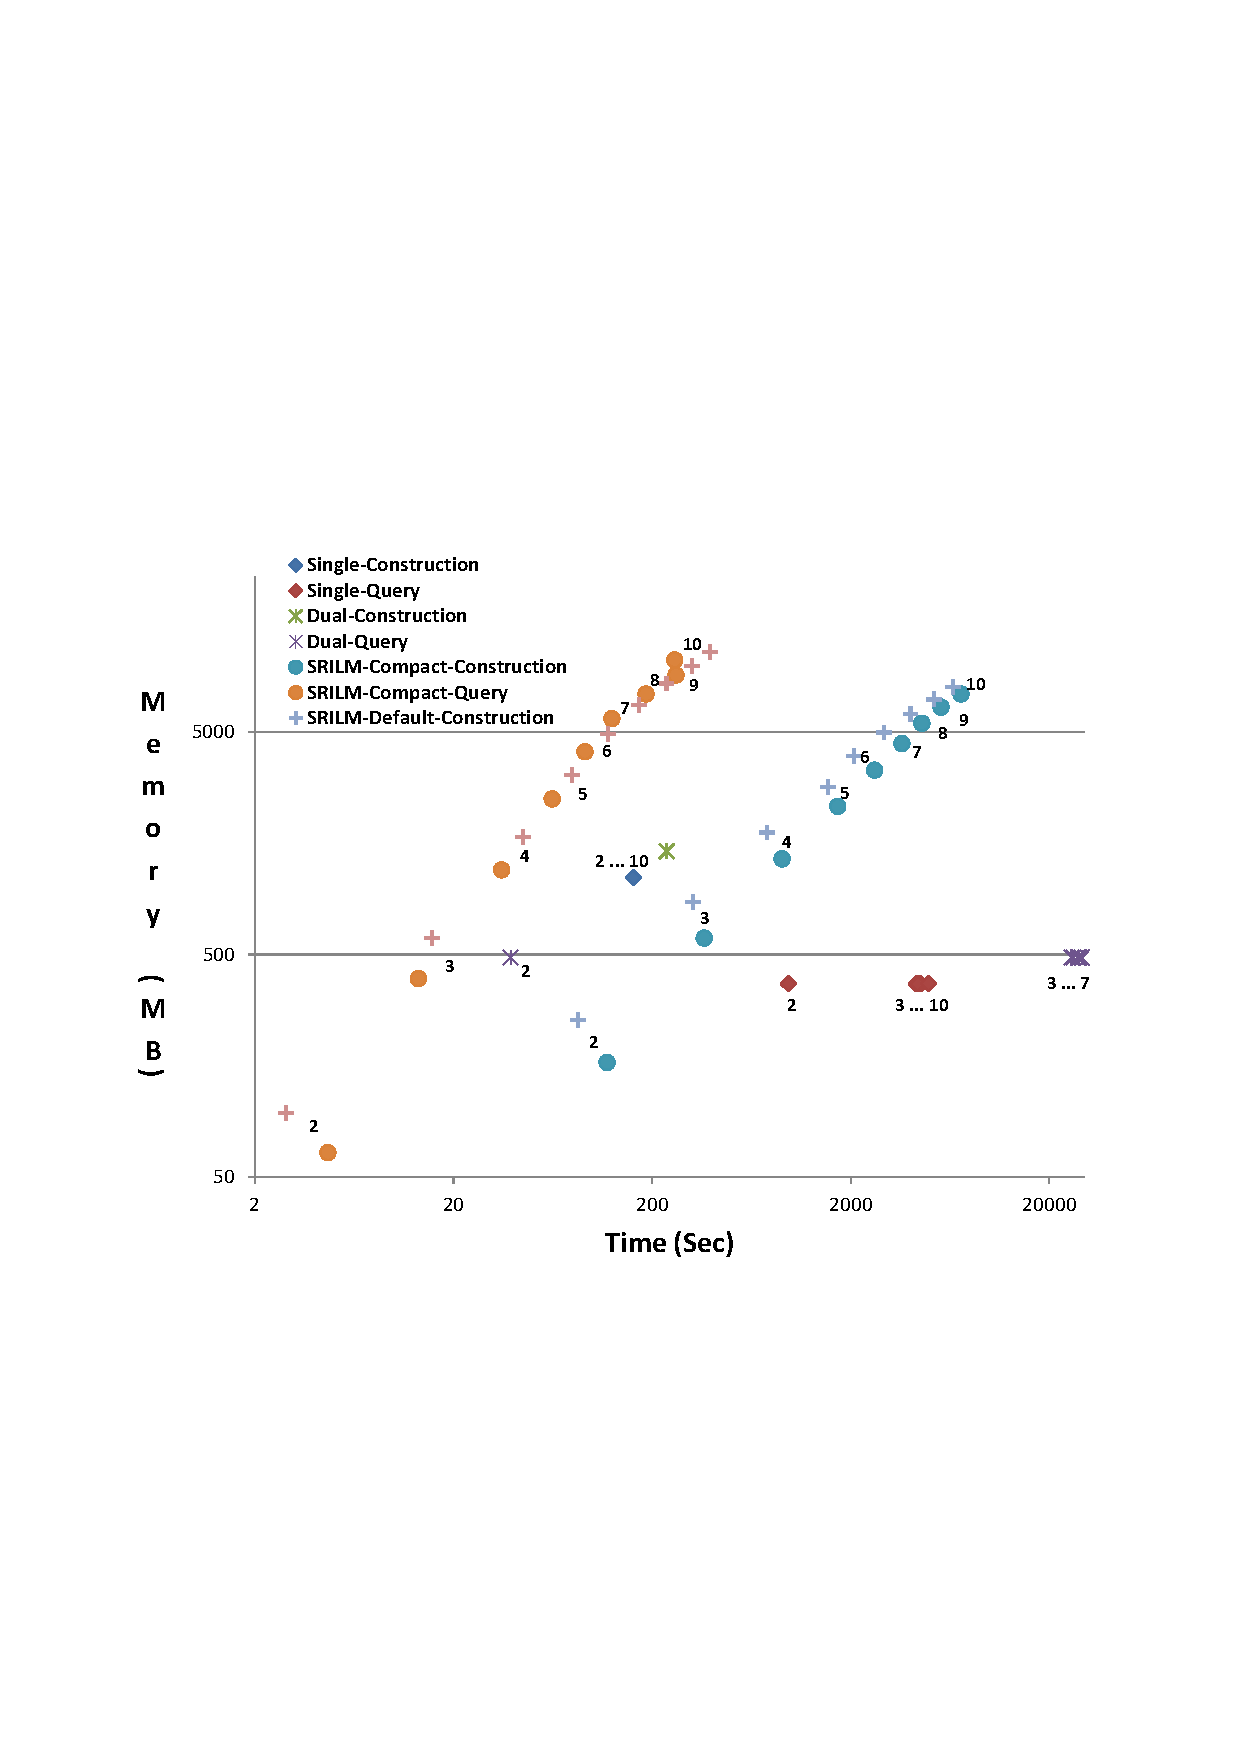
\includegraphics[width=\columnwidth]{figures/Time-Space.pdf}
\caption{On German, showing the size in MB (y axis) and time (x axis) for 4 methods: CST single, CST dual, SRILM, SRILM compact.}
\end{figure}

\missingfigure[figwidth=\columnwidth]{Wikipedia pplx (right axis), and time (left axis) for the single CST on characters vs words as a function of \ngram size.}

\missingfigure[figwidth=\columnwidth]{Wikipedia histogram over \ngram size, perhaps as a figure or table?}

\missingfigure[figwidth=\columnwidth]{Wikipedia plot (stacked bar?) of time spent in each method (n1+ x 3; backward search etc) as a function of n.}






%%% Local Variables: 
%%% mode: latex
%%% TeX-master: "cstlm"
%%% End: 



\section{Conclusions}
\label{sec-conclusions}
This paper has demonstrated the massive potential that succinct indexes have for language modelling, by developing efficient algorithms for on-the-fly computing of \ngram counts and language model probabilities.
Although we only considered a Kneser-Ney LM, our approach is portable to many other LM smoothing methods, which are formulated using similar types of count statistics.
Our complexity analysis and experimental results show favourable scaling properties with corpus size and Markov order, albeit running between 1-2 orders of magnitude slower than competitive count-based benchark LMs.
Our ongoing work seeks to close this gap: preliminary experiments suggest that with careful tuning of the succinct index parameters and precomputation, we can match or improve over the query time of \SRILM on large corpora with $m\ge6$.

%%% Local Variables: 
%%% mode: latex
%%% TeX-master: "cstlm"
%%% End: 


\bibliographystyle{acl}
\bibliography{local}

\end{document}
